%% bare_conf.tex
%% V1.4b
%% 2015/08/26
%% by Michael Shell
%% See:
%% http://www.michaelshell.org/
%% for current contact information.
%%
%% This is a skeleton file demonstrating the use of IEEEtran.cls
%% (requires IEEEtran.cls version 1.8b or later) with an IEEE
%% conference paper.
%%
%% Support sites:
%% http://www.michaelshell.org/tex/ieeetran/
%% http://www.ctan.org/pkg/ieeetran
%% and
%% http://www.ieee.org/

%%*************************************************************************
%% Legal Notice:
%% This code is offered as-is without any warranty either expressed or
%% implied; without even the implied warranty of MERCHANTABILITY or
%% FITNESS FOR A PARTICULAR PURPOSE! 
%% User assumes all risk.
%% In no event shall the IEEE or any contributor to this code be liable for
%% any damages or losses, including, but not limited to, incidental,
%% consequential, or any other damages, resulting from the use or misuse
%% of any information contained here.
%%
%% All comments are the opinions of their respective authors and are not
%% necessarily endorsed by the IEEE.
%%
%% This work is distributed under the LaTeX Project Public License (LPPL)
%% ( http://www.latex-project.org/ ) version 1.3, and may be freely used,
%% distributed and modified. A copy of the LPPL, version 1.3, is included
%% in the base LaTeX documentation of all distributions of LaTeX released
%% 2003/12/01 or later.
%% Retain all contribution notices and credits.
%% ** Modified files should be clearly indicated as such, including  **
%% ** renaming them and changing author support contact information. **
%%*************************************************************************


% *** Authors should verify (and, if needed, correct) their LaTeX system  ***
% *** with the testflow diagnostic prior to trusting their LaTeX platform ***
% *** with production work. The IEEE's font choices and paper sizes can   ***
% *** trigger bugs that do not appear when using other class files.       ***                          ***
% The testflow support page is at:
% http://www.michaelshell.org/tex/testflow/



\documentclass[conference]{IEEEtran}

\usepackage{url}
\usepackage{xspace}
\usepackage{bm}  
\usepackage{multirow}
\usepackage{multicol}
  \usepackage{amsmath}
  \usepackage{amssymb}
  \usepackage{latexsym}
  \usepackage{booktabs}
  \usepackage{amssymb}
  \setcounter{tocdepth}{3}
  \usepackage{graphicx}
  \usepackage{footnote}
  \usepackage[usenames,dvipsnames]{color}
  \usepackage{url}
  \usepackage{array}
  %\usepackage{xcolor}
  \usepackage{amsmath}
  \usepackage{breqn}
  \usepackage{comment}

  \usepackage{threeparttable, tablefootnote}
  %\usepackage[flushleft]{threeparttable}
  \usepackage{appendix}
  \usepackage{enumitem}
  \usepackage{float}
  \usepackage{setspace}

\usepackage{algorithm}
\usepackage[noend]{algpseudocode}

\usepackage{multirow}

\usepackage{enumitem}
\usepackage{subcaption}
\setlist[itemize]{noitemsep, topsep=0pt}
\newcommand{\cA}{\mathcal{A}}
\newcommand{\cB}{\mathcal{B}}
\newcommand{\cC}{\mathcal{C}}
\newcommand{\cE}{\mathcal{E}}
\newcommand{\cF}{\mathcal{F}}
\newcommand{\cH}{\mathcal{H}}
\newcommand{\cI}{\mathcal{I}}
\newcommand{\cJ}{\mathcal{J}}
\newcommand{\cL}{\mathcal{L}}
\newcommand{\cO}{\mathcal{O}}
\newcommand{\cP}{\mathcal{P}}
\newcommand{\cQ}{\mathsf{Q}}
\newcommand{\cR}{\mathsf{R}}
\newcommand{\cS}{\mathsf{S}}
\newcommand{\cU}{\mathcal{U}}
\newcommand{\cV}{\mathcal{V}}
\newcommand{\cT}{\mathsf{T}}
\newcommand{\secparameter}{\kappa}
\newcommand{\Gen}{\mathsf{Gen}}
\newcommand{\Rec}{\mathsf{Rec}}
\newcommand{\sh}{\mathsf{sh}}
\newcommand{\ie}{\textit{i.e.}}


\newcommand{\pwg}{$pwd_g$}
\newcommand{\pwv}{$pwd_v$}

%Variables
\newcommand{\pwd}{pwd}
\newcommand{\pwdg}{pwd_{g}}
\newcommand{\pwdv}{pwd_{v}}
\newcommand{\sk}{sk}
\newcommand{\vk}{vk}
\newcommand{\pp}{pp}
\newcommand{\uid}{id}
\newcommand{\sP}{\mathsf{P}}
\newcommand{\tvk}{tvk}
\newcommand{\tsk}{tsk}
\newcommand{\tpp}{tpp}
\newcommand{\vpk}{vpk}
\newcommand{\vsk}{vsk}
\newcommand{\vpp}{vpp}
\newcommand{\msg}{\mathsf{msg}}

\newcommand{\pid}{$pid$}
\newcommand{\sid}{$sid$}
%\newcommand{\secparameter}{\mathcal{K}}

\newcommand{\remove}[1]{}

\def\mg{\color{magenta}}
\def\red{\color{red}}
\def\blue{\color{blue}}
\def\green{\color{ForestGreen}}



  \usepackage[usenames,dvipsnames]{color}
  \def\red{\color{red}}
  \def\blue{\color{blue}}
  \def\magenta{\color{magenta}}
  \def\grey{\color{grey}}

  \newcommand{\SU}{\textsf{SU}}
\newcommand{\except}[1]%
{{\displaystyle \mathop{{\displaystyle}{\mathop{\ldots}^{\vee}}}^{#1}}}

\newcommand*{\QED}{\hfill\ensuremath{\blacksquare}}%

\setlength{\textfloatsep}{1\baselineskip plus 0.2\baselineskip minus 0.5\baselineskip}
\setlength{\intextsep}{10pt plus 2pt minus 2pt}

\usepackage{hyperref}
% Some Computer Society conferences also require the compsoc mode option,
% but others use the standard conference format.
%
% If IEEEtran.cls has not been installed into the LaTeX system files,
% manually specify the path to it like:
% \documentclass[conference]{../sty/IEEEtran}





% Some very useful LaTeX packages include:
% (uncomment the ones you want to load)


% *** MISC UTILITY PACKAGES ***
%
%\usepackage{ifpdf}
% Heiko Oberdiek's ifpdf.sty is very useful if you need conditional
% compilation based on whether the output is pdf or dvi.
% usage:
% \ifpdf
%   % pdf code
% \else
%   % dvi code
% \fi
% The latest version of ifpdf.sty can be obtained from:
% http://www.ctan.org/pkg/ifpdf
% Also, note that IEEEtran.cls V1.7 and later provides a builtin
% \ifCLASSINFOpdf conditional that works the same way.
% When switching from latex to pdflatex and vice-versa, the compiler may
% have to be run twice to clear warning/error messages.






% *** CITATION PACKAGES ***
%
%\usepackage{cite}
% cite.sty was written by Donald Arseneau
% V1.6 and later of IEEEtran pre-defines the format of the cite.sty package
% \cite{} output to follow that of the IEEE. Loading the cite package will
% result in citation numbers being automatically sorted and properly
% "compressed/ranged". e.g., [1], [9], [2], [7], [5], [6] without using
% cite.sty will become [1], [2], [5]--[7], [9] using cite.sty. cite.sty's
% \cite will automatically add leading space, if needed. Use cite.sty's
% noadjust option (cite.sty V3.8 and later) if you want to turn this off
% such as if a citation ever needs to be enclosed in parenthesis.
% cite.sty is already installed on most LaTeX systems. Be sure and use
% version 5.0 (2009-03-20) and later if using hyperref.sty.
% The latest version can be obtained at:
% http://www.ctan.org/pkg/cite
% The documentation is contained in the cite.sty file itself.






% *** GRAPHICS RELATED PACKAGES ***
%
\ifCLASSINFOpdf
  % \usepackage[pdftex]{graphicx}
  % declare the path(s) where your graphic files are
  % \graphicspath{{../pdf/}{../jpeg/}}
  % and their extensions so you won't have to specify these with
  % every instance of \includegraphics
  % \DeclareGraphicsExtensions{.pdf,.jpeg,.png}
\else
  % or other class option (dvipsone, dvipdf, if not using dvips). graphicx
  % will default to the driver specified in the system graphics.cfg if no
  % driver is specified.
  % \usepackage[dvips]{graphicx}
  % declare the path(s) where your graphic files are
  % \graphicspath{{../eps/}}
  % and their extensions so you won't have to specify these with
  % every instance of \includegraphics
  % \DeclareGraphicsExtensions{.eps}
\fi
% graphicx was written by David Carlisle and Sebastian Rahtz. It is
% required if you want graphics, photos, etc. graphicx.sty is already
% installed on most LaTeX systems. The latest version and documentation
% can be obtained at: 
% http://www.ctan.org/pkg/graphicx
% Another good source of documentation is "Using Imported Graphics in
% LaTeX2e" by Keith Reckdahl which can be found at:
% http://www.ctan.org/pkg/epslatex
%
% latex, and pdflatex in dvi mode, support graphics in encapsulated
% postscript (.eps) format. pdflatex in pdf mode supports graphics
% in .pdf, .jpeg, .png and .mps (metapost) formats. Users should ensure
% that all non-photo figures use a vector format (.eps, .pdf, .mps) and
% not a bitmapped formats (.jpeg, .png). The IEEE frowns on bitmapped formats
% which can result in "jaggedy"/blurry rendering of lines and letters as
% well as large increases in file sizes.
%
% You can find documentation about the pdfTeX application at:
% http://www.tug.org/applications/pdftex





% *** MATH PACKAGES ***
%
%\usepackage{amsmath}
% A popular package from the American Mathematical Society that provides
% many useful and powerful commands for dealing with mathematics.
%
% Note that the amsmath package sets \interdisplaylinepenalty to 10000
% thus preventing page breaks from occurring within multiline equations. Use:
%\interdisplaylinepenalty=2500
% after loading amsmath to restore such page breaks as IEEEtran.cls normally
% does. amsmath.sty is already installed on most LaTeX systems. The latest
% version and documentation can be obtained at:
% http://www.ctan.org/pkg/amsmath





% *** SPECIALIZED LIST PACKAGES ***
%
%\usepackage{algorithmic}
% algorithmic.sty was written by Peter Williams and Rogerio Brito.
% This package provides an algorithmic environment fo describing algorithms.
% You can use the algorithmic environment in-text or within a figure
% environment to provide for a floating algorithm. Do NOT use the algorithm
% floating environment provided by algorithm.sty (by the same authors) or
% algorithm2e.sty (by Christophe Fiorio) as the IEEE does not use dedicated
% algorithm float types and packages that provide these will not provide
% correct IEEE style captions. The latest version and documentation of
% algorithmic.sty can be obtained at:
% http://www.ctan.org/pkg/algorithms
% Also of interest may be the (relatively newer and more customizable)
% algorithmicx.sty package by Szasz Janos:
% http://www.ctan.org/pkg/algorithmicx




% *** ALIGNMENT PACKAGES ***
%
%\usepackage{array}
% Frank Mittelbach's and David Carlisle's array.sty patches and improves
% the standard LaTeX2e array and tabular environments to provide better
% appearance and additional user controls. As the default LaTeX2e table
% generation code is lacking to the point of almost being broken with
% respect to the quality of the end results, all users are strongly
% advised to use an enhanced (at the very least that provided by array.sty)
% set of table tools. array.sty is already installed on most systems. The
% latest version and documentation can be obtained at:
% http://www.ctan.org/pkg/array


% IEEEtran contains the IEEEeqnarray family of commands that can be used to
% generate multiline equations as well as matrices, tables, etc., of high
% quality.




% *** SUBFIGURE PACKAGES ***
%\ifCLASSOPTIONcompsoc
%  \usepackage[caption=false,font=normalsize,labelfont=sf,textfont=sf]{subfig}
%\else
%  \usepackage[caption=false,font=footnotesize]{subfig}
%\fi
% subfig.sty, written by Steven Douglas Cochran, is the modern replacement
% for subfigure.sty, the latter of which is no longer maintained and is
% incompatible with some LaTeX packages including fixltx2e. However,
% subfig.sty requires and automatically loads Axel Sommerfeldt's caption.sty
% which will override IEEEtran.cls' handling of captions and this will result
% in non-IEEE style figure/table captions. To prevent this problem, be sure
% and invoke subfig.sty's "caption=false" package option (available since
% subfig.sty version 1.3, 2005/06/28) as this is will preserve IEEEtran.cls
% handling of captions.
% Note that the Computer Society format requires a larger sans serif font
% than the serif footnote size font used in traditional IEEE formatting
% and thus the need to invoke different subfig.sty package options depending
% on whether compsoc mode has been enabled.
%
% The latest version and documentation of subfig.sty can be obtained at:
% http://www.ctan.org/pkg/subfig




% *** FLOAT PACKAGES ***
%
%\usepackage{fixltx2e}
% fixltx2e, the successor to the earlier fix2col.sty, was written by
% Frank Mittelbach and David Carlisle. This package corrects a few problems
% in the LaTeX2e kernel, the most notable of which is that in current
% LaTeX2e releases, the ordering of single and double column floats is not
% guaranteed to be preserved. Thus, an unpatched LaTeX2e can allow a
% single column figure to be placed prior to an earlier double column
% figure.
% Be aware that LaTeX2e kernels dated 2015 and later have fixltx2e.sty's
% corrections already built into the system in which case a warning will
% be issued if an attempt is made to load fixltx2e.sty as it is no longer
% needed.
% The latest version and documentation can be found at:
% http://www.ctan.org/pkg/fixltx2e


%\usepackage{stfloats}
% stfloats.sty was written by Sigitas Tolusis. This package gives LaTeX2e
% the ability to do double column floats at the bottom of the page as well
% as the top. (e.g., "\begin{figure*}[!b]" is not normally possible in
% LaTeX2e). It also provides a command:
%\fnbelowfloat
% to enable the placement of footnotes below bottom floats (the standard
% LaTeX2e kernel puts them above bottom floats). This is an invasive package
% which rewrites many portions of the LaTeX2e float routines. It may not work
% with other packages that modify the LaTeX2e float routines. The latest
% version and documentation can be obtained at:
% http://www.ctan.org/pkg/stfloats
% Do not use the stfloats baselinefloat ability as the IEEE does not allow
% \baselineskip to stretch. Authors submitting work to the IEEE should note
% that the IEEE rarely uses double column equations and that authors should try
% to avoid such use. Do not be tempted to use the cuted.sty or midfloat.sty
% packages (also by Sigitas Tolusis) as the IEEE does not format its papers in
% such ways.
% Do not attempt to use stfloats with fixltx2e as they are incompatible.
% Instead, use Morten Hogholm'a dblfloatfix which combines the features
% of both fixltx2e and stfloats:
%
% \usepackage{dblfloatfix}
% The latest version can be found at:
% http://www.ctan.org/pkg/dblfloatfix




% *** PDF, URL AND HYPERLINK PACKAGES ***
%
%\usepackage{url}
% url.sty was written by Donald Arseneau. It provides better support for
% handling and breaking URLs. url.sty is already installed on most LaTeX
% systems. The latest version and documentation can be obtained at:
% http://www.ctan.org/pkg/url
% Basically, \url{my_url_here}.




% *** Do not adjust lengths that control margins, column widths, etc. ***
% *** Do not use packages that alter fonts (such as pslatex).         ***
% There should be no need to do such things with IEEEtran.cls V1.6 and later.
% (Unless specifically asked to do so by the journal or conference you plan
% to submit to, of course. )


% correct bad hyphenation here
\hyphenation{op-tical net-works semi-conduc-tor}


\begin{document}
%
% paper title
% Titles are generally capitalized except for words such as a, an, and, as,
% at, but, by, for, in, nor, of, on, or, the, to and up, which are usually
% not capitalized unless they are the first or last word of the title.
% Linebreaks \\ can be used within to get better formatting as desired.
% Do not put math or special symbols in the title.
\title{Threshold Password-based Token Validation in Single-Sign On Systems}


% author names and affiliations
% use a multiple column layout for up to three different
% affiliations
\author{\IEEEauthorblockN{Michael Shell}
\IEEEauthorblockA{School of Electrical and\\Computer Engineering\\
Georgia Institute of Technology\\
Atlanta, Georgia 30332--0250\\
Email: http://www.michaelshell.org/contact.html}
\and
\IEEEauthorblockN{Homer Simpson}
\IEEEauthorblockA{Twentieth Century Fox\\
Springfield, USA\\
Email: homer@thesimpsons.com}
\and
\IEEEauthorblockN{James Kirk\\ and Montgomery Scott}
\IEEEauthorblockA{Starfleet Academy\\
San Francisco, California 96678--2391\\
Telephone: (800) 555--1212\\
Fax: (888) 555--1212}}

% conference papers do not typically use \thanks and this command
% is locked out in conference mode. If really needed, such as for
% the acknowledgment of grants, issue a \IEEEoverridecommandlockouts
% after \documentclass

% for over three affiliations, or if they all won't fit within the width
% of the page, use this alternative format:
% 
%\author{\IEEEauthorblockN{Michael Shell\IEEEauthorrefmark{1},
%Homer Simpson\IEEEauthorrefmark{2},
%James Kirk\IEEEauthorrefmark{3}, 
%Montgomery Scott\IEEEauthorrefmark{3} and
%Eldon Tyrell\IEEEauthorrefmark{4}}
%\IEEEauthorblockA{\IEEEauthorrefmark{1}School of Electrical and Computer Engineering\\
%Georgia Institute of Technology,
%Atlanta, Georgia 30332--0250\\ Email: see http://www.michaelshell.org/contact.html}
%\IEEEauthorblockA{\IEEEauthorrefmark{2}Twentieth Century Fox, Springfield, USA\\
%Email: homer@thesimpsons.com}
%\IEEEauthorblockA{\IEEEauthorrefmark{3}Starfleet Academy, San Francisco, California 96678-2391\\
%Telephone: (800) 555--1212, Fax: (888) 555--1212}
%\IEEEauthorblockA{\IEEEauthorrefmark{4}Tyrell Inc., 123 Replicant Street, Los Angeles, California 90210--4321}}




% use for special paper notices
%\IEEEspecialpapernotice{(Invited Paper)}




% make the title area
\maketitle

% As a general rule, do not put math, special symbols or citations
% in the abstract
\begin{abstract}
Single-Sign On (SSO) systems permit an {\em identity provider (IdP)} to authenticate a user with a password %$pwd_a$ 
and issue them a token for authentication to a {\em relying party (RP)} (e.g. a website that the user would like to access). The RP %trusts the IdP and can 
authenticates the user by verifying the IdP's signature on the user's token. This is an attractive solution to password-based authentication over the Internet because the user authenticates to different services with a single password. Tokens, however, can be stolen while transmitted over the network or stored and processed on the user's device, then used to impersonate the user to the RP without compromising their password. Proof-of-Possession (PoP) tokens resist token stealing but require a secure element on the user's device to store a secret key. %must be kept confidential while stored or transmitted because they can be stolen and be presented by anyone to impersonate the user to the RP.

We propose a new type of token called Proof-of-Password (PoPwd) that requires the user to demonstrate knowledge of a password to the RP. Our PoPwd tokens provide protection against stealing and do not require the user to store any long-term secrets or pre-register any information with the RP. We formalize and prove security of PoPwd token generation and token validation.

We also provide a proof-of-concept implementation of PbDTV and compare it to two other commonly used token systems that we implemented, and show feasibility and advantages of our system in practice.

\end{abstract}

% no keywords




% For peer review papers, you can put extra information on the cover
% page as needed:
% \ifCLASSOPTIONpeerreview
% \begin{center} \bfseries EDICS Category: 3-BBND \end{center}
% \fi
%
% For peerreview papers, this IEEEtran command inserts a page break and
% creates the second title. It will be ignored for other modes.
\IEEEpeerreviewmaketitle



\section{Introduction}
Passwords are widely used for user authentication where the user registers a unique public identifier (username) and a password that is a low-entropy
secret with a server, and can later authenticate itself by using the same password in the authentication protocol. If the server is compromised, the stored password information is vulnerable to {\em offline dictionary attacks} that can recover the password \cite{camenisch2015optimal,cryptoeprint:2019/199}.
Users are known to choose weak passwords and use related passwords for multiple accounts, and so a breach at one server is dangerous for the security of others \cite{hanamsagar2018leveraging}.

{\em Single-Sign-On (SSO) systems}, like OPID \cite{openIDConnect} and SAML \cite{SAML}, allow users to register a username and password with a single authentication server called {\em identity provider (IdP)}, and then use the IdP 
to authenticate themselves to a third party server referred to as the {\em relying party (RP)} who the user does not have any prior registration with.
When the user wants to login to an RP,  their request is redirected to the IdP. The user authenticates itself to the IdP with their registered password and receives a {\em bearer token} \cite{rfc6750} 
that consists of (i) a message $m$ that describes context information, and (ii) the digital signature of IdP on $m$ \cite{SAML,jwt-rfc7519}.
The user presents the token to the RP who {\em validates the token} by verifying the digital signature using the IdP's verification key, and if accepted, processes the context information. SSO systems are attractive because they (SSO1) let users authenticate to many RPs using a single registered password, and (SSO2) compromise of the RP does not leak the password. A major vulnerability of the system however is the possibility of {\em token stealing} when the token is transmitted over the network, or stored and processed on the user's device \cite{MicrosoftTokenTheft,GitHubTokenTheft}. The attacker can simply copy the token and use it to impersonate the user to the RP without breaking security of user-to-Idp authentication.

%
A widely used protection against token stealing is embedding an expiration time in the message part of the token, specifying a {\em validity period} for the token. The length of validity period must balance the threat of token stealing against the frequency of the user's authentication to the RP. Bearer tokens are usually one-time use and have short validity periods. One-time tokens however require the user to re-authenticate to the IdP in every access to the RP, which will be inefficient when the same RP must be contacted frequently. Also, in the event that the IdP is unavailable, the user cannot access the RP altogether.

{\em Proof-of-Possession (PoP) tokens} \cite{rfc8705}  are multiple-use tokens that provide protection against token stealing. 
A user with a pair of public and private keys ($pk_{U},sk_{U}$) obtains a token that embeds $pk_{U}$ as part of the message. 
To authenticate itself to an RP, the user must ``prove" that they know the corresponding private key. %of $pk_{U}$. 
This is by (i) presenting the token to the RP, then (ii) digitally signing a random challenge that is sent to them by the RP, using $sk_{U}$. PoP tokens have two attractive properties: (i) they decouple token generation and token validation processes.  That is, the user does not need to interact with the IdP when it needs to contact the RP, and (ii) protects against token stealing because token validation requires the presenter to demonstrate knowledge of $sk_{U}$.\\ 
PoP tokens however have two major restrictions: (i) the user's device requires a secure element to store $sk_{U}$, and (ii) tokens are bound to the device with the secure element. If the user has multiple devices, the secret key needs to be synchronized between them which may not be straightforward, %can be cumbersome for the user and 
increasing the risk of key compromise.

In this paper, we consider a new type of token that we call {\em Proof-of-Password (PoPwd) } tokens, and  use  passwords instead of public and  private keys for protection against token stealing. To our knowledge, this is the first attempt to use passwords to {\em protect the token}. Using passwords for token protection has numerous advantages. Passwords are memorizable secrets, and  so PoPwds will have the advantages of PoP token but  remove the user's need to employ a secure element, allowing the user to easily synchronize their tokens between multiple devices. Additionally, passwords are easier to generate and update, and a wide variety of password managers that can safely store and synchronize the password %are available that simplify storage and synchronization 
across multiple devices, allowing the token to be used on any device of the user's choice.
%for uses that require this.

There is however a significant challenge in implementing this approach because of the possibility of offline password attacks. PoPwd tokens embed a function of the password (FoP) $pwd_v$, that is $f(pwd_{v}), $ in the token $m$. The embedded information will be used during a token presentation protocol %to the RP, 
to convince the RP that the user knows $pwd_{v}$. The FoP embedded in the token's message, and the process of PoPwd token validation must be secure against offline attacks on $pwd_{v}$.

In \cite{HalveiKrawczyk99,Impagliazzo88} it is argued that preventing offline dictionary attacks against password-based protocols without using public-key techniques, would require the user to pre-register a large shared secret with the RP which would negate the need for an SSO system in the first place (and will require secure element). 
Using approaches such as embedding a randomized commitment %\cite{Pedersen91} 
to $pwd_{v}$ in $m$ using a high-entropy random  $r$, requires the user to securely store $r$ and protect it from leaking. 

A solution that comes close to our goal is based on the encrypted challenge-response protocols of \cite{Boyarsky99,HalveiKrawczyk99} for user authentication. The RP will publish a public key for a secure encryption system, that the user will use to encrypt $pwd_{v}$ and embed it in the token. A user can then demonstrate their knowledge of $pwd_{v}$ with a challenge-response protocol.% will be used to demonstrate the user's knowledge of $pwd_{v}$.  
This approach removes the need for the user to have a secure element or store secrets on its device.

This solution however %(i) 
does not protect $pwd_{v}$ if the RP's secret key is compromised (in which case all $pwd_v$s of users will be compromised)%, and (ii)  has the inconvenience of the need for the user to obtain the public key of the RP before a token request to IdP is made.
In the following we further elaborate %more 
on this challenge and how our design address it.


\noindent{\bf \textit{Our Work}.}
We introduce and formalize the notion of a {\em Password-based Distributed Token Validation (PbDTV)} scheme for PoPwd tokens. PbDTV is a cryptographic protocol that allows distributed validation of  PoPwds, and enjoys a number of attractive properties including not requiring user registration to the validation servers and security against offline password attacks.\\
We use PbDTV to contruct a {\em distributed token validation service} (dTkVS) that will %be used by RPs and 
offload the token validation process of RPs to the service (a concept similar to offloading authentication to IdP) and remains transparent to the user. The dTkVS consists of $n$ servers %and provides token validation as a service to the RP 
and has the following properties: 

- S1: The validation service can validate an IdP issued token without the need to interact with the IdP and can be used for any IdP. %from  a wide variety of IdPs who are not required to be online during token validation. 
%We only 
The only requirement is that the IdP encodes user defined values in the token's message in a standard way, for example using existing SSO standards  (\cite{openIDConnect,SAML}).
The user does not need to register with the dTkVS or the RP.

- S2: The token's password $pwd_v$ remains secure even if the RP and up to $t-1$ dTkVS servers are compromised.\\
The service remains available as long as $t$ validation servers are up and running.

-S3: The service can be used by any RP who knows the public keys of the dTkVS's $n$ servers and completely outsources the computation for the RP. 
This makes the service particularly attractive to resource constrained IoT devices that need to validate access tokens but desire strong authentication guarantees.


\begin{figure}
\centering
\begin{subfigure}{.4\textwidth}
  \centering
  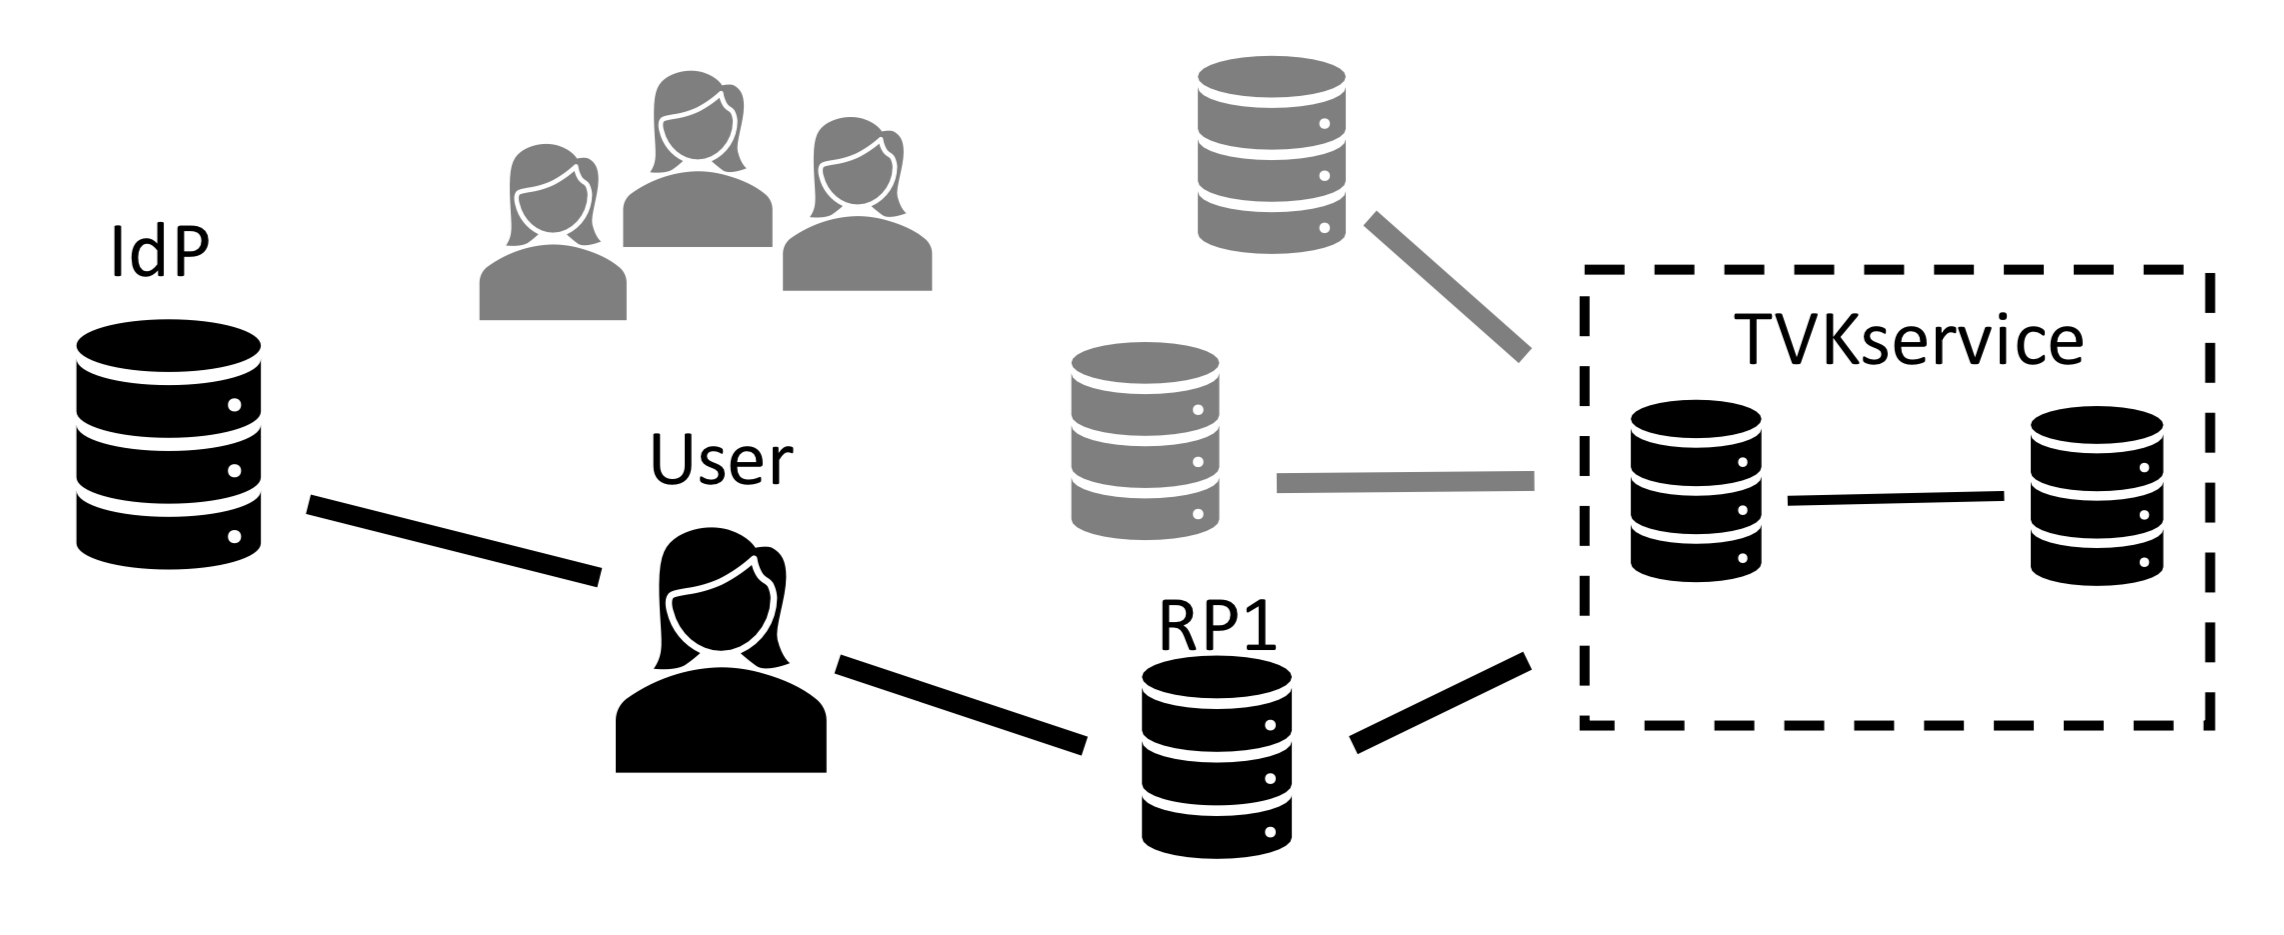
\includegraphics[width=\textwidth]{Figures/general.jpeg}
  \caption{High-level View}
  \label{fig:sub1}
\end{subfigure}%
\begin{subfigure}{.6\textwidth}
  \centering
  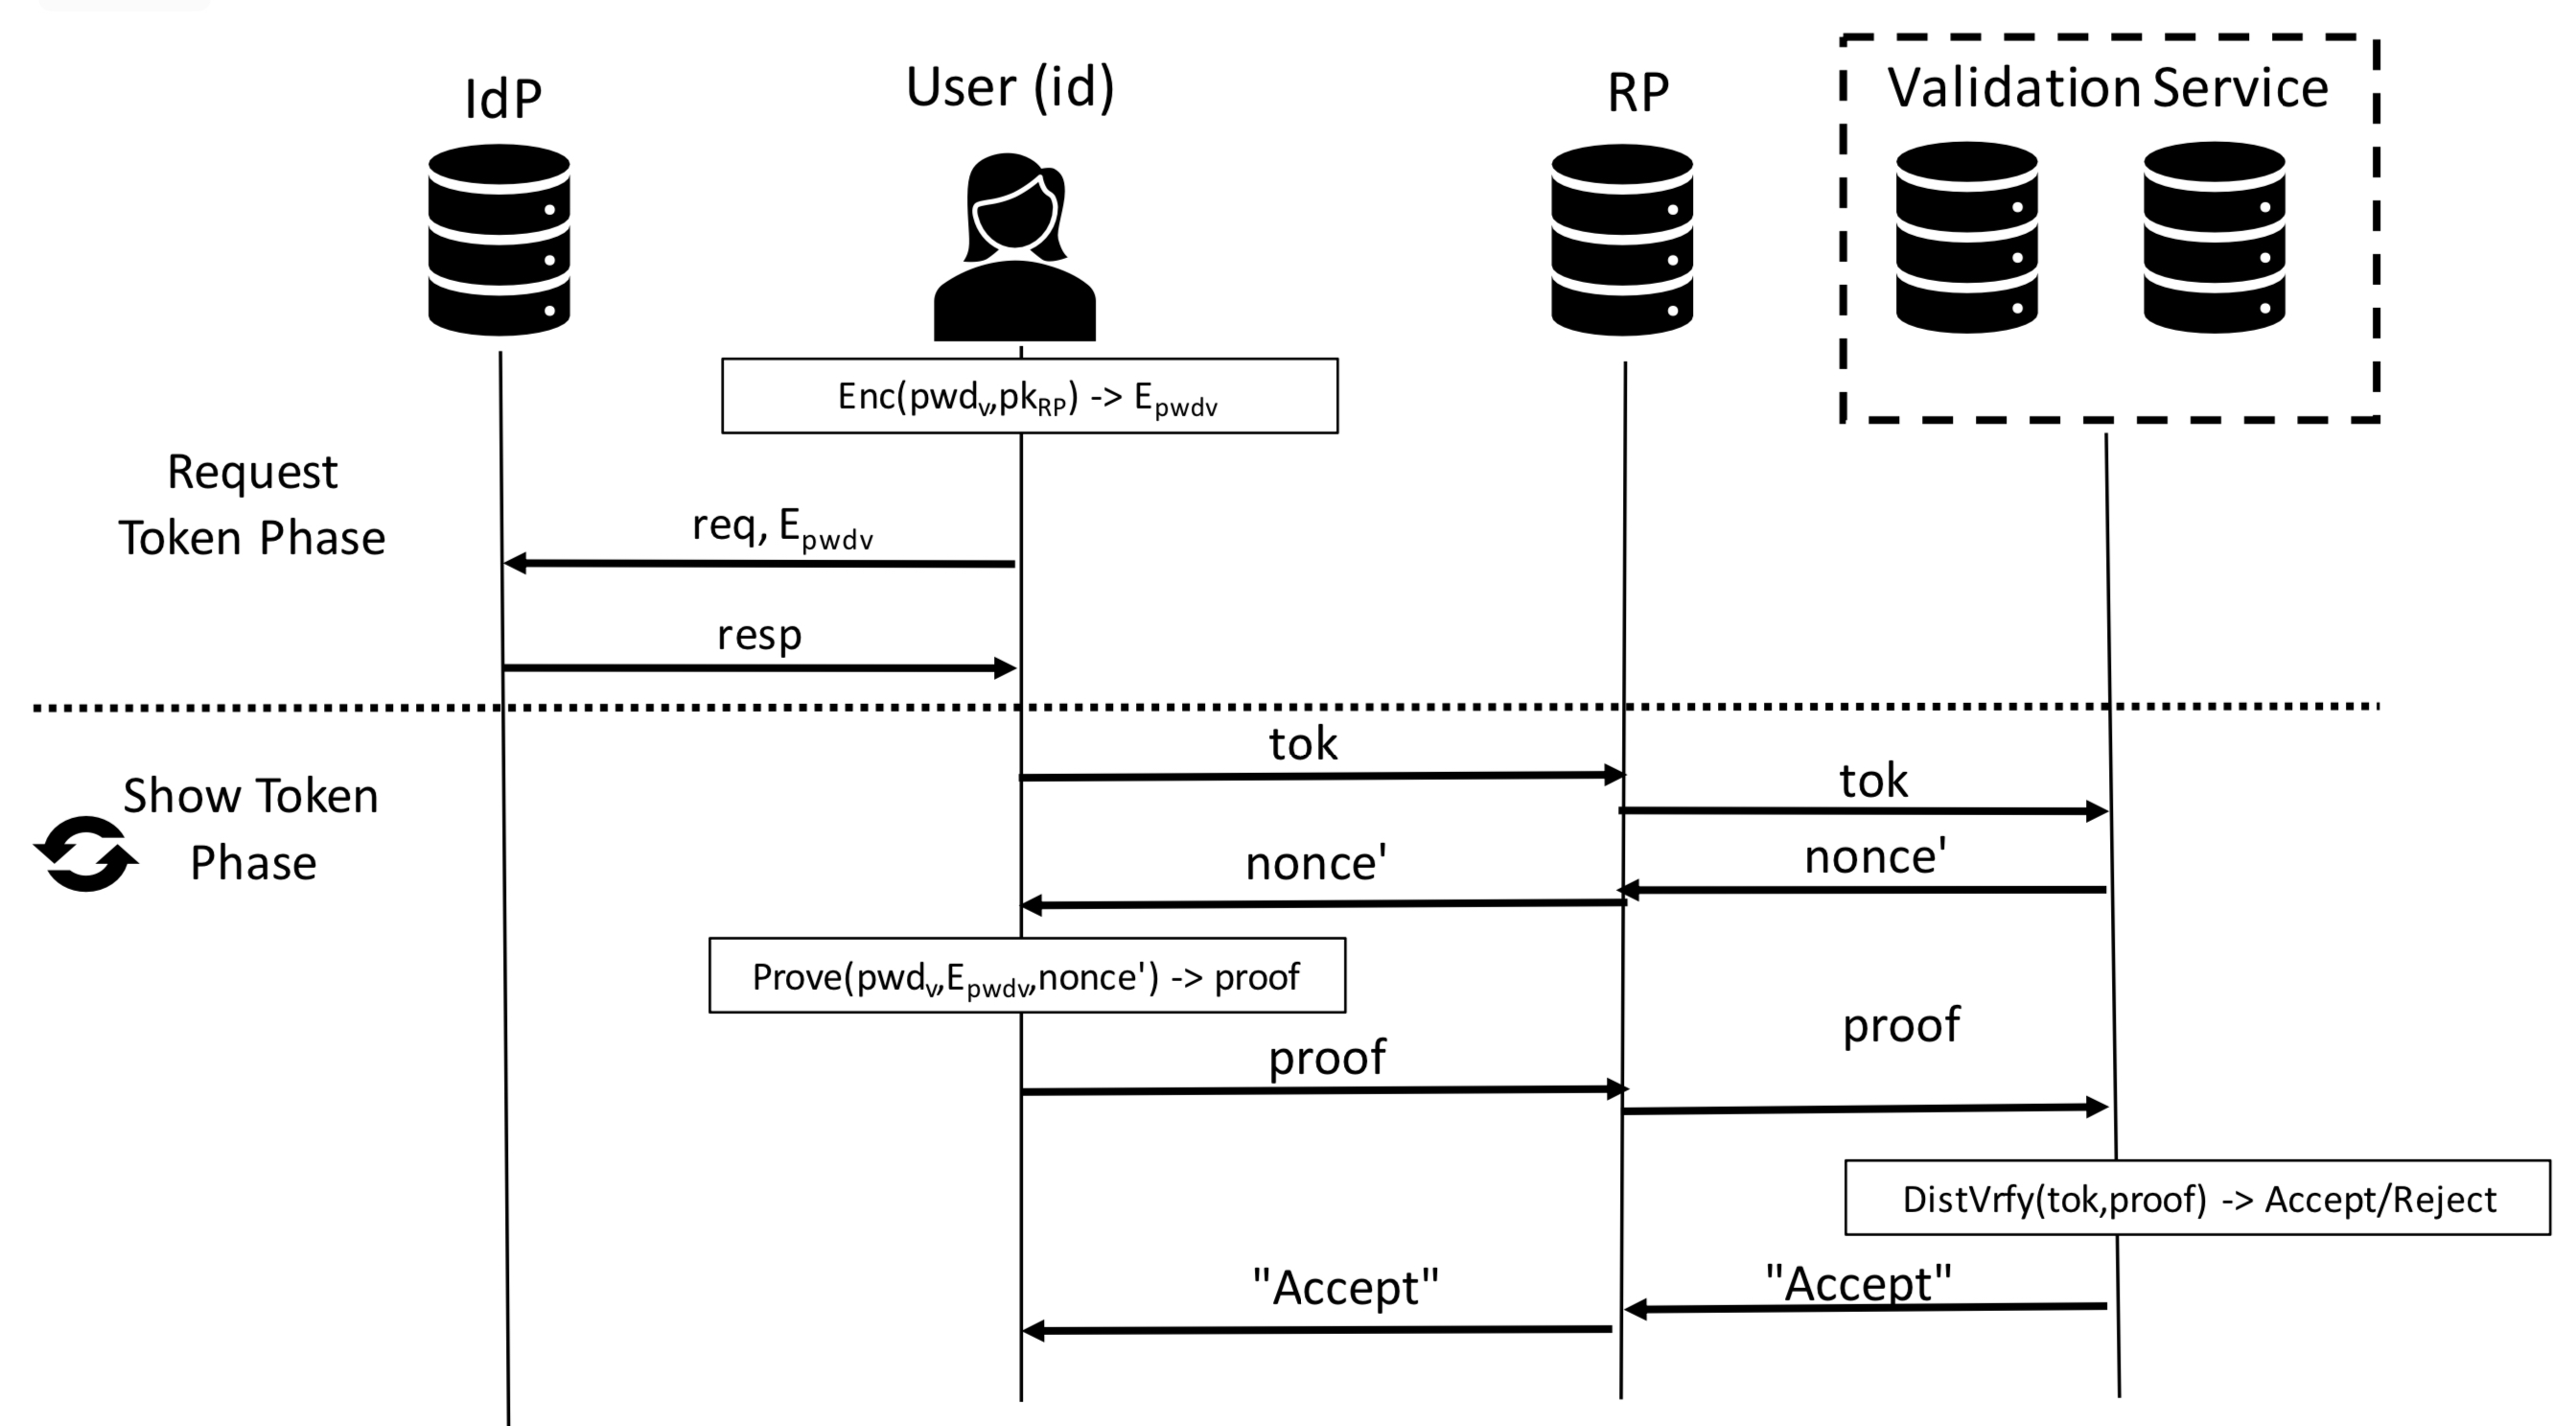
\includegraphics[width=\textwidth]{Figures/sequencePbDTV.jpeg}
  \caption{Message flow of the dTkVS system. Request Token and Show Token phases are depicted.}
  \label{fig:sub2}
\end{subfigure}
\caption{Distributed Token Validation Service (dTkVS) extension to an SSO system}
\label{PbDTVFlow}
\end{figure}


Figure \ref{PbDTVFlow} shows the interaction of the user with the IdP to obtain a PoPwd token, and the interactions of the user, RP, and token validation service to validate the token. The user only needs to interact with the RP who then interacts with the dTkVS as a token validation backend. Details of the interaction is in Section \ref{PbDTV-Body}. The result of token validation by the dTkVS (Acc/Rej) will be provided to the RP over an authenticated channel.

Thus PoPwd tokens will have the token protection benefits of PoP tokens, all the user-side benefits of using passwords, and protection against offline password attacks. Outsourcing token validation to the dTkVS relieves the RP from performing any computation
making it a compelling design. Figure \ref{token-compare} compares different types of tokens and shows that our PoPwd tokens are the only ones to achieve all the desired properties.

\begin{figure}
\begin{centering}
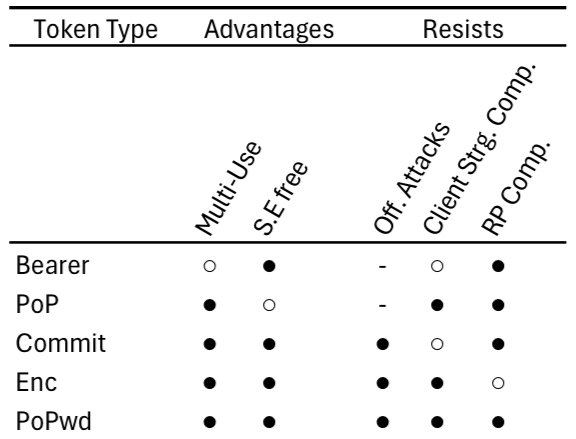
\includegraphics[width=.5\textwidth]{Figures/TableCompare.jpeg}
\caption{Comparison of different token types.}
\label{token-compare}
\end{centering}
\end{figure}

\noindent{\bf \textit{Our Contribution}.}
%{\em PbDTV:} 
We propose PbDTV, a cryptographic protocol for  {\em $t$-out-of-$n$ distributed validation of PoPwd tokens} where validation servers have the signature verification key of the IdP. We give a game-based formal security model that captures a powerful attacker who can steal user tokens, and has full control over the network to view, modify, add, or delete messages. We define two security properties for the model:  {\em Token-Impersonation resistance} that ensures the attacker cannot forge tokens or use stolen ones unless it knows the correct password that is embedded in the token. As an attacker can always request validation of a stolen PoPwd, similar to all password-based cryptographic protocols, we require that the best an attacker can do is to
to perform this online guessing attack with the goal of correctly guessing the user's passwords.  The second security property is
{\em Token-Password Safety} that protects the embedded password in the PoPwd from offline dictionary attacks.

Our construction of the distributed token validation protocol is inspired by the distributed verification protocol used in the construction of the password authenticated key exchange protocol \cite{T-PAKE-Mackenzie},  and its security relies on  the hardness of the Decisional Diffie-Hellman problem.
The protocol works as follows. The $n$ validation servers have a semantically secure 
public key encryption system with public key $pk_{pbdtv}$ that provides threshold decryption. The public key is securely provided to the user (e.g. in a certificate). The user selects a password $pwd_v$ that is used for protection of its tokens, maps it
to an element of $\mathbb{Z}^{*}_{q}$ and encrypts the multiplicative inverse $(pwd_{V})^{-1}$ under servers public, key obtaining $E_{pwd_{v}}= Enc_{pk_{pbdtv}}((pwd_{v})^{-1})$. The user requests  a token from the IdP that embeds $Enc_{pk_{pbdtv}}((pwd_{v})^{-1})$ in the token's message. %and receives a signed token with the requested message.
%encryption embeded in the token' message.
The token can be stored on the user's device without the need for extra protection.
To use the token for accessing a service, 
the user presents the token and generates a ``proof" that it knows $pwd_v$.  This is by applying a transformation on the token that ``cancels out" $(pwd_{v})^{-1}$ in $E_{pwd_{v}}$. A set of $t$ validation servers will verify the IdP's signature on the token, and once verified, run a distributed decryption protocol to check if the transformation was computed successfully. %$B$ is an encryption of 1. 
To prevent leakage of information about $pwd_{v}$ we use simulation-sound \cite{814628} non-interactive zero-knowledge proofs (SS-NIZK) where a party can demonstrate they know the secrets used to construct their messages and have the required security properties for password-based protocols \cite{cryptoeprint:2014/429}. We use the same SS-NIZK proofs from \cite{T-PAKE-Mackenzie} and refer there for their full description. %for the discrete log relationships between ElGamal ciphertexts.

In our security analysis we consider the most stringent (from security view point) case that IdP is also password based. The security model of PbDTV includes an IdP that has the user registered with a password $pwd_a$, and allows the adversary to query IdP. This models composition of token issuing and token presentation. For extreme security analysis we allow $pwd_a = pwd_v$ and require password safety against the adversary with oracle access to issuing and verification.\\

Our password-based token generation protocol and its formalization of security is described next.\\

{\bf Token generation:} We design and formalize a password-based token generation (PbTG) scheme that uses {\em implicit user authentication} to the IdP. Implicit authentication provides an efficient way to protect token generation with passwords that are safe from offline dictionary attacks. In implicit authentication, the IdP does not verify the request from the user. Rather they process and respond to every request they receive according to the claimed user $id$ with the associated stored password $pwd^{id}_{a}$. Only the user who knows $pwd^{id}_{a}$ can recover a valid token. Implicit authentication ensures that a full token can only be recovered from the response if the correct password was used.  
Implicit authentication was used in PASTA \cite{PASTA-Agrawal}, an SSO system with distributed IdP that protects user password information against IdP compromise. Although \cite{PASTA-Agrawal}, and other distributed IdP systems like \cite{PESTO-baum,PASTAU-Rawat} have nice properties, the only SSO systems deployed today we are aware of use a centralized IdP server \cite{openIDConnect,SAML}. Recall that our main contribution is the design of PbDTV to protect against token stealing after tokens are recovered by the user. To show that PbDTV is compatible with existing SSO deployments, we consider and design a centralized IdP called PASCA, that provides implicit authentication.  

{\bf Library Implementation \& Experiments} We implement a PbDTV Token Showing library for JSON Web Tokens (JWT) that are used in deployed SSO systems \cite{openIDConnect,SAML}. We run experiments by running the token showing process on simulated LAN and WAN networks. We measure the computation and communication overhead for different total servers $n$ and threshold $t$ values. Our results show the feasibility of using passwords to protect tokens where the user experiences a delay of under $0.5$ seconds when $(t=2,n=2)$. Additionally, user-side computation is only \%25 percent more compared to PoP tokens which is a limited computational cost in exchange for the PoP's secure element. 

\noindent
{\bf Paper organization:} Section \ref{sec:preliminaries} provides preliminary background. Section \ref{sec:PbTG} and \ref{sec:PbDTV} are descriptions of our password-based IdP and PbDTV, including security model and constructions with proved  security.
%Section \ref{sec:ring-token-anonymity-body} is on token anonymity that is provided by our password-based IdP. 
We describe our implementation and experiments in Section \ref{sec:Implementation} and conclude the paper in Section \ref{sec:Conclusion}.


\vspace{1mm}
\noindent {\it \textbf{Related Work.}}
Passwords have a huge body of research on their construction and analysis
\cite{camenisch2015optimal,chakraborty2022honeyword,everspaugh2015pythia}. 
Defence against online-guessing attacks can be achieved by rate limiting login attempts. Offline attacks can be slowed with salting and memory-hard hashing \cite{cryptoeprint:2016/100,cryptoeprint:2017/442,7536388}, but once enough information is gathered to confirm password guesses offline the password should be considered compromised.

Recent SSO systems PASTA \cite{PASTA-Agrawal} and PESTO \cite{PESTO-baum} protect the user's password from server compromise by distributing the IdP among $n$ different servers. Both protocols are provably secure even when some of the $n$ servers are corrupted and allow the user to obtain a bearer token only if they know the correct password. The security properties ensure that user passwords remains unknown, even to the IdP, and tokens cannot be generated unless a user knows the correct password. However, there are no protections for the token after the user recovers it. The best an adversary who controls the network and corrupts some issuers can do to learn the password is online guessing attacks against the IdP. Both protocols have trusted setup and registration phases and require confidential channels during token verification, but only PESTO requires confidential channels during token issuing. 

Another SSO scheme \cite{cryptoeprint:2023/915} in the distributed IdP setting allows private attribute-based token issuing. For each user attribute, the IdP servers store a randomized secret value and the user stores a secret attribute key. The user and a threshold of servers evaluate the user's attributes on a given policy by running a multiparty computation (MPC) over the user's secret attribute keys and the IdP's randomized values. Anyone with the correct attribute keys can receive a bearer token. This scheme requires user-side secure storage and confidential channels for the secret attribute keys and for the issued bearer-tokens. Privacy here ensures the IdP remain oblivious to the user's attributes as long as no more than a threshold of servers are corrupt, but the identity of the requesting user is necessarily known to IdP.   %protects the user's attributes but the IdP servers must know the identity of the requesting user. 
%Depending on what information is included in the token's structured message, they may have a privacy property called \emph{unlinkability from colluding RPs} where different RPs working together cannot determine if two or more tokens were created for the same user.   

The above SSO systems require at least some of the IdP servers to be online for the user to log into the RP making it easier for the IdP to track the user's access patterns. Some privacy-aware SSO systems address this by masking the identity of the RP during the user's login to the IdP through randomized RP identifiers \cite{10.1145/3605760.3623767,10.1145/3320269.3384724,guo2022uppresso} or mixing services that hide which RP the user logs into among many other RPs \cite{10190538}. 
%$Other systems protect user access patterns from the IdP by decoupling the user's authentication to the IdP from the credential showing to the RP. These systems replace the bearer token with a long-lived verifiable credential that can be shown multiple times without the need to interact with the IdP \cite{8422732,Zhang_2021,10.1145/3605760.3623767}. However, all these systems require confidential-storage on the user side or none hide the user identity from the IdP. 

%{\blue insert paragraph about privacy notions in token showing protocols}

Self Sovereign Identity (SSI) systems use verifiable credentials to give the user full ownership over their credentials (i.e. only the user who was issued the credential can use it) and full control over how their credential is used (i.e. the user doesn't need to interact with any other entity when showing their credentials to an RP). In practice such systems require a trade-off   

The verifiable credentials encode identity and attribute information.  and are used to generate multiple showing poofs that their attributes satisf. These proofs reveal nothing about the user's attributes except that they are satisfied. These solutions all require use-side confidential storage for large entropy secrets.     

Token theft has been identified as a major concern. Existing solutions rely on secure storage \cite{10.1007/978-3-642-19125-1_7}\cite{10.1145/1367497.1367568}, or specialized token access control \cite{10.3233/JCS-150529}. These solutions do not protect tokens after they are leaked. 

Passwords have been used for other applications like authenticated key exchange (PAKE) \cite{bellovin}, its thresholdized version (T-PAKE) \cite{T-PAKE-Mackenzie,di2003provably}, and password-protected secret sharing (PPSS) 
\cite{PPSS-bagherzand,jarecki2014round} but none of these systems can be directly applied for protecting tokens. A previous scheme \cite{5670871} uses passwords to protect tokens while in storage but is vulnerable to token validator compromise and stealing while tokens are transmitted. 

Other works propose passwordless user authentication with biometrics or public-key infrastructure (PKI) instead of an SSO system. Biometrics replace passwords with scans of physical characteristics \cite{mock2012real,10.1145/2382196.2382307}
but server breaches now leak personally identifiable information creating huge privacy risks. FIDO \cite{FIDO} has a promising system for PKI-based user authentication where security relies on secure elements for key storage and both require the user to pre-register with each server they access. Research has begun formalizing their security \cite{Bindel2022} and privacy is largely left as an open problem. Usability issues \cite{9152694} suggest passwords will still play an important role in the future.

\section{Preliminaries}
\label{sec:preliminaries}

Security parameter is denoted by $\secparameter$. Square brackets around an integer $[n]$ denote the set of integers $\{1,\ldots,n\}$. We assume \pwv=\pwg~ and refer to both with $\pwd$ although our definitions can be extends for \pwv$\neq$\pwg.
%

\noindent
{\bf Digital Signature Scheme:} A UF-CMA digital signature scheme $\mathsf{SIG}$ is a tuple of three algorithms $(\mathsf{KGen}, \mathsf{Sign}, \mathsf{Verify})$. We use the traditional UF-CMA signatures \cite{10.1137/0217017} and the definition can be found in Appendix \ref{appndx:prelim_SS}.

\noindent
{\bf Oblivous Pseudo-random Functions}
We use the 2HashDH oblivious pseudo-random function (OPRF) from \cite{7467360} and adapt to the game-based model using the same techniques in \cite{PASTA-Agrawal} for adapting the threshold OPRF from \cite{Jarecki2017TOPPSSCP}. A $(\mathcal{X},\mathcal{R})$-oblivious pseudo-random function (OPRF) $\mathsf{OP}$ is a tuple of PPT algorithms ($\mathsf{Setup}$, $\mathsf{Encode}$, $\mathsf{Eval}$, $\mathsf{Compute}$) that satisfies correctness below.
\\
$\mathsf{Setup}$ $(1^{\secparameter}$) $\rightarrow (sk,pp)$. Generates a secret key $sk$ and public parameters $pp$.\\
$\mathsf{Encode}(x,\rho) \leftarrow c$. Generates an encoding $c \in \mathcal{X}$ using randomness $\rho \in R$.\\
$\mathsf{Eval}(sk,c) := z$. Evaluates the $\mathsf{OP}$ on the encoded value $c$ using the secret key $sk$.\\
$\mathsf{Compute}(x,z,\rho) := h/\perp$. Finalizes the computation of the $\mathsf{OP}$ using randomness $\rho$ to generate value $h$. If algorithm fails, its output is denoted by $\perp$.\\
%
\noindent{\em Correctness}. For all $\secparameter \in \mathbb{N}$ all $(sk,pp)$ generated by Setup($1^{\secparameter}$), and value $x \in X$, and randomness $\rho, \rho' \in R$, if $c \leftarrow \mathsf{Encode}(x, \rho$), $c' \leftarrow \mathsf{Encode}(x, \rho'$), $z :=  \mathsf{Eval}(sk, c$) and $z' := \mathsf{Eval}(k,c'$), then $\mathsf{Compute}(x,z,\rho) = \mathsf{Compute}(x, z', \rho'$).
\\

The $\mathsf{OP}$ has {\em Unpredictability} and {\em Obliviousness}. Unpredictability implies that it is hard for an adversary to predict the output of $\mathsf{OP}$ on a challenge input $\tilde{x}$. More specifically, the adversary can view a polynomial number of partial evaluations on $\tilde{x}$, $c,z$, and still their best strategy is to make a guess for $\tilde{x}$ and compute the output through an oracle call. Obliviousness implies that the output of $\mathsf{OP}$ leaks only a negligible amount about a challenge input $\tilde{x}$. An adversary can view a polynomial number of partial evaluations, $c,z$ and the $\mathsf{OP}$ output $h$ on challenge input $\tilde{x}$, but their best strategy is to make a guess for $\tilde{x}$ and verify it through an oracle call.
\\
{\em $2HashDH$ Construction}  with input space $\mathcal{X}$.
\begin{itemize}
\item $\mathsf{Setup}(1^{\secparameter})$. Run $\mathsf{GroupGen}(1^{\secparameter})$ to get $(p,g,\mathbb{G})$. Pick a $sk$ at random from $Z_{p}$. Let $H_1: X \times G \rightarrow \{0,1\}^{\secparameter}$ and $H_2: X \times G \rightarrow \mathbb{G}$ be hash functions. Output $k$ and pp $:= (p,g,\mathbb{G},H_1,H_2)$.
\item $\mathsf{Encode}(x,\rho$). Output $H_2(x)^{\rho} := c$
\item $\mathsf{Eval}(sk,c)$. Output $c^{sk} := z$
\item $\mathsf{Compute}(x,z,\rho$).  Output $H_1(x||z^{\rho^{-1}})$.
\end{itemize}
%
 \noindent{\bf Theorem 1:} 2HashDH is an $\mathsf{OP}$ Security is formalized and proven with straightforward modifications of the proofs in \cite{PASTA-Agrawal}. The main differences are that we use the One-More Diffie-Hellman (OMDH) instead of the Gap Threshold (OMDH), and the adversary only needs to make a single oracle query, instead of $t$ separate queries, to verify a guesses about $\tilde{x}$. Formal proofs are deferred to our full paper for space.

\section{PASCA: Password-based Centralized Authentication}
\label{sec:PbTG}

We first define the syntax and security of a password-based Token Generation (PbTG) scheme, then describe our construction PASCA that achieves the defined security. A PbTG system has a token issuer $IdP$ and any number of users $\uid$ and has 4 phases: {\em Setup}, {\em Register}, {\em Request}, and {\em Verification}. The PbTG only requires that a use know their password to obtain a token. We discuss security details in the next subsection. 
 
\noindent {\bf password-based Token Generation}
\label{def:PbTG}
A PbTG scheme $\Upsilon$ for a password space $\mathsf{P}$ is a tuple of PPT algorithms $(\mathsf{Setup}$, $\mathsf{SignUp}$, $\mathsf{Store}$, $\mathsf{Request}$, $\mathsf{Response}$, $\mathsf{Recover}$, $\mathsf{Verify})$ that satisfies the correctness property.
\\
\noindent \underline{1. {\em Setup Phase}:} initialization of the $IdP$.\\
$\mathsf{Setup}(1^{\secparameter}) \rightarrow (\sk,\vk,\pp)$: On input a security parameter $1^{\secparameter}$ and password space $\mathsf{P}$, outputs a public verification key $\vk$, secret signing key $\sk$, and public parameters $\pp$. The $\pp$ is an implicit input to all other algorithms in this system.\\
\noindent \underline{2. {\em Registration Phase}:} where users select a password and send a registration request to the $IdP$ who creates and stores a registration record;\\
\noindent $\mathsf{SignUp}(\uid,\pwd) \rightarrow msg$: Run by the user $\uid$ with their selected password $\pwd \in \sP$. It outputs a registration message $msg$.\\
\noindent $\mathsf{Store}(\uid,msg) \rightarrow \bot / rec_{\uid}$: Run by $IdP$. Input is a registration message $msg$ and outputs a registration record that is stored in $\mathsf{Rec}[\uid] = rec_{\uid}$. If a record for $\uid$ already exists, output $\bot$.\\
\noindent \underline{3. {\em Request Token Phase}:} lets registered users choose a message $m$ and request a token that embeds $m$ from the $IdP$.\\
\noindent $\mathsf{Request}(\uid,\pwd,m) \rightarrow (st, req)$: Run by user with password $\pwd$, and message $m$. Outputs a request message $req$ and state $st$.\\      
\noindent $\mathsf{Response}(\sk, \uid, m, req) \rightarrow \bot / resp$: Run by the $IdP$.\\
The $IdP$ uses $\mathsf{Rec}[\uid]$, the request $req$, and the secret key $\sk$ to create a response $resp$. If $\mathsf{Rec}[\uid] = \perp$, output $\perp$.\\
\noindent $\mathsf{Recover}(st, resp) \rightarrow \bot / tok_{\uid,m}$: Run by user on response from $IdP$ and local state $st$. Outputs a token $tok_{\uid,m}$ or $\bot$ if no token was recovered.\\
\noindent \underline{4. {\em Verification Phase:}} checks that the token is valid under the $IdP$'s public verification key.\\
$\mathsf{Verify}(\vk, tok_{\uid,m}) \rightarrow 0/1$: Input $tok_{\uid,m}$ and $IdP$'s verification key $\vk$. If the token is valid, the algorithm outputs $1$, otherwise outputs $0$.\\
\noindent {\bf Correctness:} For all $\secparameter \in \mathbb{N}$, any password space $\mathsf{P}$, and all $(\sk, \vk, \pp)$ generated by $\mathsf{Setup}(1^{\secparameter})$, any user $\uid$, any password $\pwd \in \sP$, any message $m$: {\em If} a user $id$ runs the {\em Registration} phase with $pwd$ and later runs the {\em Request Token} phase claiming to be $id'=id$ with $pwd'=pwd$ and requesting a token that embeds $m$, {\em then} the user will be able to obtain token $tok_{id,m}$ that successfully verifies under $IdP$'s $\vk$.  

We capture concurrent and sequential executions and denote the $i$-th instance of user $\uid$ with $\pi^{i}_{\uid}$. Since PbTG has implicit user authentication, each run of the response algorithm represents a new instance of $IdP$ so we suppress the notation in this case for brevity.

\subsection{Security} 
A PbTG scheme is secure if it satisfies two properties: (i) \emph{password-safety} implies an attacker's advantage in guessing a user's password is negligibly better than performing online-dictionary attacks even when they learn other user's passwords and (ii) \emph{unforgeability} where it is infeasible for anyone to obtain a valid token for user $\uid$ without knowing their password. 


\vspace{1mm}
\noindent
{\bf Password-safety and Unforgeability.}
We assume the $IdP$ remains incorruptable and that users know their public token verification key. Adversary $\cA$ adaptively corrupts users to learn their password. Registration is done over a confidential channel (TLS in practice) which is captured with the single registration oracle. The adversary has complete network control in the {\em Request Token} phase captured with separate oracles for each algorithm. When $\cA$ queries the response oracle as $\uid$ with a request that was not honestly generated by the request oracle, a counter $q_{\uid}$ is incremented. Another counter $q_{\uid,m}$ is incremented every time the response oracle is queried on $\uid$ and $m$.
The password-safety and unforgeability of a PbTG scheme is defined with the following security game.


%\begin{figure}
%\begin{centering}
%\includegraphics[width=\textwidth]{Figures/PbTGGame.jpeg}
%\caption{PbTG Game}
%\label{token_compare}
%\end{centering}
%\end{figure}


\noindent {\bf PbTG Security Game: }$\mathsf{SecGame}_{\Upsilon, \cA}(1^{\secparameter, \sP, w})$
\label{obtain-game}
\begin{multicols}{2}
\raggedright
\scriptsize
 
\noindent $\mathsf{Setup}(1^{\secparameter}) \rightarrow (\vk,\sk,\pp)$.\\        
        %\item $\cA$ selects a target user $\uid^{T}$: $(\uid^{T}, st_{\cA}) \longleftarrow \cA(\pp)$.
$(\uid^{T}, st_{\cA}) \longleftarrow \cA(\pp)$.\\
$q_{\uid} := 0$ and $\mathsf{TOKS}_{\uid} = \emptyset$ for all users $\uid$.\\
$q_{\uid,m} := 0$ for all $\uid$ and $m$.\\    
$\mathsf{Sessions}_{\uid}, \mathsf{Pwds}, \mathsf{Rec} = []$,
\\
$\mathsf{COR}, \mathsf{REQS}, \mathsf{TOKS} = \emptyset$,
\\ 
$out \leftarrow \cA^{\langle \cO \rangle}(st_{\cA})$\\         
\end{multicols}


\begin{multicols}{2}
\raggedright
\scriptsize
\noindent {\bf Oracles:}\\
\noindent \underline{$\cO_{register}(\uid)$} %\rightarrow 0/1$: 
A password for $\uid$ is selected uniformly at random from the password space $\pwd_{\uid} \xleftarrow{\$} \sP$ and a registration record is created and stored in $\mathsf{Rec}[\uid] = rec_{\uid}$. Then set $\mathsf{Pwds}[\uid] = \pwd$.\\     
\noindent \underline{$\cO_{corrupt}(\uid)$} %\rightarrow \bot / \pwd_{\uid}$: 
$\cA$ can corrupt users to learn their password. { Oracle} Returns $\mathsf{Pwds}[\uid]$ if a record for $\uid$ exists and $\bot$ otherwise. Adds $\uid$ to $\mathsf{COR}$.\\ 
\noindent \underline{$\cO_{request}(\uid,i,m)$} %\rightarrow \perp/req$: 
If $\mathsf{Pwds}[\uid] \neq \perp$ and instance $\pi^{i}_{\uid}$ was not used before, then $\uid$'s password is used to generate a request. The resulting state is saved in $\mathsf{Sessions}_{\uid}[i] = \perp$ and $req$ is added to $\mathsf{REQS}_{\uid}$. If $i$ was used already output $\perp$.\\
\noindent \underline{$\cO_{response}(\uid,m,req)$} %\rightarrow \perp/resp$: 
The oracle uses the inputs and $\mathsf{Rec}[\uid]$ to generate response $resp$. To keep track of confirm-able password guesses made by $\cA$ the counter $q_{\uid}$ is incremented by $1$ when $req \notin \mathsf{REQS}_{\uid}$. $q_{\uid,m}$ is incremented by $1$ on every invocation.\\
\noindent \underline{$\cO_{recover}(\uid,i,m,resp)$} %\rightarrow \perp/tok_{\uid,m}$: 
State $\mathsf{Sessions}_{\uid}[i]$ is used with $resp$ to attempt to recover a token. If a token $tok_{\uid,m}$ is successfully recovered it is added to $\mathsf{TOKS}$. Outputs $\perp$ if no token is recovered.
\end{multicols}



%\begin{definition}[Password-Safety]
\noindent
{\bf Password-Safety:}
    \label{def:password_safety_PbTG} 
    A PbTG scheme $\Upsilon$ satisfies \textbf{Password-Safety} if for all password spaces $\sP$ and all PPT adversaries $\cA$ in $\mathsf{SecGame}_{\Upsilon,\cA}(1^{\secparameter},\sP)$, there exists a negligible function $\mathsf{negl}$ such that
    
    \[Pr[ \uid^{T} \notin \mathsf{COR} \land out = \mathsf{Pwds}[\uid^{T}] \neq \bot] \leq ~ \frac{q_{\uid^T} + 1}{|\sP|} + \mathsf{negl}(\secparameter)\]

%\end{definition}
     Here, $out$ is a password guess for target user $\uid^{T}$ that $\cA$ may not have previously verified with the oracles (additive factor of $1$).
    
    %\begin{definition}[Unforgeability of Tokens]\label{def:unforge_PbTG}
    \noindent
    {\bf Unforgeability:}\label{def:unforge_PbTG}
    A PbTG scheme $\Upsilon$ has \textbf{Unforgeability} if for all password spaces $\sP$ and PPT adversaries $\cA$ in $\mathsf{SecGame}_{\Upsilon,\cA}(1^{\secparameter},\sP)$, there exists a negligible function $\mathsf{negl}$ such that
    
    if $q_{\uid^{T},m^{T}} < 1$ then 
    \[Pr[\mathsf{Verify}(\vk,tok_{\uid^{T},m^{T}})] \leq \mathsf{neg}(\secparameter)\]
    
    else:
    \[Pr[ \uid^{T} \notin \mathsf{COR} \land tok_{\uid^{T},m^{T}} \notin \mathsf{TOKS} \land \mathsf{Verify}(\vk,tok_{\uid^{T},m^{T}})] \leq ~ \frac{q_{\uid^{T}}}{|\sP|} + \mathsf{negl}(\secparameter)\]
%    \end{definition}
    $\cA$'s output is a token $tok_{\uid^{T},m^{T}}$ with embedded message $m^{T}$ for user $\uid^{T}$. The two winning conditions are first, the response oracle did not generate the token $tok_{\uid^{T}}$ and $\cA$'s advantage should be negligible. In the second case, $\cA$ recovers $tok_{\uid^{T},m^{T}}$ that was generated by the response oracle but not output by the recover oracle and their advantage in forging a token is dominated by their advantage in guessing $\uid^{T}$'s password.

%\subsubsection{Ring-token-anonymity}
    
%\end{definition}

\subsection{PASCA Construction}
 
PASCA, Figure \ref{pasca-construction}, outlines a way to combine a UF-CMA secure digital signature scheme $\mathsf{SIG}$, oblivious pseudo-random function (OPRF) $\mathsf{OP},$ %satisfying unpredictability and obliviousness defined in Section \ref{sec:preliminaries} and Appendix \ref{appx-oprf},
{\em  symmetric-key encryption} scheme $\mathsf{SKE}$, and a hash function $H$ to build a PbTG scheme that achieves our security guarantees.

%\begin{theorem}\label{thm:PASCA-security}
    \noindent{\bf Theorem 2:} If $\mathsf{SIG}$ is unforgeable, $\mathsf{OP}$ is unpredictable and oblivious, and $\mathsf{SKE}$ is a CPA-secure symmetric-key encryption scheme, then the PbTG scheme PASCA described in Fig. \ref{pasca-construction} has password-safety and, unforgeability when $H$ is modeled as a random oracle.
%\end{theorem}

%Proof for Theorem 1 is in Appendix
\noindent
{\em Proof Sketch.}
The proof for Theorem 2 is derived from a straightforward modification of the hybrid argument proofs for PASTA \cite{PASTA-Agrawal} where the reduction is to the our OPRF instead of \cite{PASTA-Agrawal}'s threshold OPRF. The main difference is that the adversary in PASCA only needs to make one oracle query to check a password guess instead of $t$ different queries in PASTA. Another small difference in our PASCA proof compared to PASTA is we do not need to rely on authenticated channels in the token issuing phase as long as the user knows the correct token verification key. We omit the formal proof due to the space constraint.
%\ref{sec:Appndx_proof_PASCA}.


\begin{figure*}
\begin{multicols}{2} \raggedcolumns
\scriptsize
\underline{{\bf Primitives:}}
\begin{itemize}
    \item %Signature Scheme: 
    $\mathsf{SIG}$ := ($\mathsf{KGen}, \mathsf{Sign}, \mathsf{Verify}$)
    \item %Oblivious PRF: 
    $\mathsf{OP}$ := ($\mathsf{Setup}, \mathsf{Encode}, \mathsf{Eval}, \mathsf{Compute})$
    \item %Symmetric-Key Encryption scheme: 
    $\mathsf{SKE} := (\mathsf{Enc}, \mathsf{Dec})$
    \item Hash function $H$
\end{itemize}

\vspace{3mm}
\underline{{\em1. Setup:}}\\
$\mathsf{Setup}(1^{\secparameter}) \rightarrow (\sk, \vk, \pp)$ \hspace*{\fill} (Server) 
\begin{itemize}
    \item $(\sk,\vk, spp) \xleftarrow{\$} \mathsf{SIG.KGen}(1^{\secparameter})$ 
    \item $\pp := (\secparameter, P, spp)$ 
\end{itemize}
\underline{{\em2. Registration:}}\\
$\mathsf{SignUp}(\uid, \pwd$) $\rightarrow (\uid,msg)$ \hspace*{\fill} (User)
\begin{itemize}
    \item  $(k,opp) \xleftarrow{\$} \mathsf{OP.Setup}(1^{\secparameter}$) 
    \item  $h := \mathsf{OP}(k,\pwd$) and $h' := H(h)$
    \item  $msg := (k,h')$ %{\hspace{5mm}\mg (Given to the Server) }
\end{itemize}

$\mathsf{Store}(\uid, msg) \rightarrow (rec_{\uid})$ \hspace*{\fill} (Server)
\begin{itemize}
    \item Parse $msg$ as $(k,h')$
    \item $rec_{\uid} := (k,h')$
    \item $\mathsf{Rec}[\uid] = rec_{\uid}$
\end{itemize}

\columnbreak
\underline{{\em3. Request Token:}}\\
$\mathsf{Request}(\uid,\pwd) \rightarrow (req,st,m)$ \hspace*{\fill} (User)
\begin{itemize}
    \item $\rho \xleftarrow{\$} \mathbb{Z}_{p}$
    \item $c \leftarrow \mathsf{OP.Encode}(\pwd, \rho)$.
    \item $req := c$ and $st =: (\uid, \pwd, \rho)$
    \item return $req$
\end{itemize}

%\columnbreak

$\mathsf{Respond}(\sk, \uid, m ,req$) $\rightarrow (res)$ \hspace*{\fill} (Server)
\begin{itemize}
    \item If $\mathsf{Rec}[\uid] = \perp$ return $\perp$. Otherwise, parse $rec_{\uid}$ as $(k,h)$
    \item $z \leftarrow \mathsf{OP.Eval}(k, req)$
    \item $sig \xleftarrow{\$} \mathsf{SIG.Sign}(\sk,\uid||m$)
    \item return $res := (z, \mathsf{SKE.Enc}(h,sig))$
\end{itemize}

$\mathsf{Recover}(st,res) \rightarrow tok_{\uid,m}$ \hspace*{\fill} (User)
\begin{itemize}
    \item Parse $res$ as $(z,ctxt)$ and $st$ as $(\uid, pwd, \rho)$
    \item $h \leftarrow \mathsf{OP.Compute}(pwd, z,\rho)$ and $h' := H(h)$
    \item $sig \leftarrow \mathsf{SKE.Dec}(h',ctxt)$
    \item return $tok_{\uid,m} := (sig,\uid||m)$
\end{itemize}

\underline{{\em4. Verification:}}\\
$\mathsf{Verify}(vk,tok_{\uid,m}) \leftarrow 0/1$ \hspace*{\fill} (Implicit Verifier)
\begin{itemize}
    \item Parse $tok_{\uid,m} = (sig,\uid||m)$
    \item return $\mathsf{SIG.Verify}(\vk,\uid||m,sig)$ 
\end{itemize}
%\end{minipage}
\end{multicols}
%}
\caption{PASCA Construction}
\label{pasca-construction}
\end{figure*}

% An example of a floating figure using the graphicx package.
% Note that \label must occur AFTER (or within) \caption.
% For figures, \caption should occur after the \includegraphics.
% Note that IEEEtran v1.7 and later has special internal code that
% is designed to preserve the operation of \label within \caption
% even when the captionsoff option is in effect. However, because
% of issues like this, it may be the safest practice to put all your
% \label just after \caption rather than within \caption{}.
%
% Reminder: the "draftcls" or "draftclsnofoot", not "draft", class
% option should be used if it is desired that the figures are to be
% displayed while in draft mode.
%
%\begin{figure}[!t]
%\centering
%\includegraphics[width=2.5in]{myfigure}
% where an .eps filename suffix will be assumed under latex, 
% and a .pdf suffix will be assumed for pdflatex; or what has been declared
% via \DeclareGraphicsExtensions.
%\caption{Simulation results for the network.}
%\label{fig_sim}
%\end{figure}

% Note that the IEEE typically puts floats only at the top, even when this
% results in a large percentage of a column being occupied by floats.


% An example of a double column floating figure using two subfigures.
% (The subfig.sty package must be loaded for this to work.)
% The subfigure \label commands are set within each subfloat command,
% and the \label for the overall figure must come after \caption.
% \hfil is used as a separator to get equal spacing.
% Watch out that the combined width of all the subfigures on a 
% line do not exceed the text width or a line break will occur.
%
%\begin{figure*}[!t]
%\centering
%\subfloat[Case I]{\includegraphics[width=2.5in]{box}%
%\label{fig_first_case}}
%\hfil
%\subfloat[Case II]{\includegraphics[width=2.5in]{box}%
%\label{fig_second_case}}
%\caption{Simulation results for the network.}
%\label{fig_sim}
%\end{figure*}
%
% Note that often IEEE papers with subfigures do not employ subfigure
% captions (using the optional argument to \subfloat[]), but instead will
% reference/describe all of them (a), (b), etc., within the main caption.
% Be aware that for subfig.sty to generate the (a), (b), etc., subfigure
% labels, the optional argument to \subfloat must be present. If a
% subcaption is not desired, just leave its contents blank,
% e.g., \subfloat[].


% An example of a floating table. Note that, for IEEE style tables, the
% \caption command should come BEFORE the table and, given that table
% captions serve much like titles, are usually capitalized except for words
% such as a, an, and, as, at, but, by, for, in, nor, of, on, or, the, to
% and up, which are usually not capitalized unless they are the first or
% last word of the caption. Table text will default to \footnotesize as
% the IEEE normally uses this smaller font for tables.
% The \label must come after \caption as always.
%
%\begin{table}[!t]
%% increase table row spacing, adjust to taste
%\renewcommand{\arraystretch}{1.3}
% if using array.sty, it might be a good idea to tweak the value of
% \extrarowheight as needed to properly center the text within the cells
%\caption{An Example of a Table}
%\label{table_example}
%\centering
%% Some packages, such as MDW tools, offer better commands for making tables
%% than the plain LaTeX2e tabular which is used here.
%\begin{tabular}{|c||c|}
%\hline
%One & Two\\
%\hline
%Three & Four\\
%\hline
%\end{tabular}
%\end{table}


% Note that the IEEE does not put floats in the very first column
% - or typically anywhere on the first page for that matter. Also,
% in-text middle ("here") positioning is typically not used, but it
% is allowed and encouraged for Computer Society conferences (but
% not Computer Society journals). Most IEEE journals/conferences use
% top floats exclusively. 
% Note that, LaTeX2e, unlike IEEE journals/conferences, places
% footnotes above bottom floats. This can be corrected via the
% \fnbelowfloat command of the stfloats package.

\section{Distributed Token Validation Service (dTkVS)}
\label{sec:PbDTV}
Our dTkVS provides PoPwd token validation as a back-end service to multiple RPs. The system is built using our PbDTV scheme. We first formalize the notion of a PbDTV and present a security model to define the desired security properties {\em Token-Password Safety} and {\em Token-Impersonation Resistance} in a multi-user setting. We then propose a construction based on our description above that uses our PbTG scheme for the IdP and token issuance. We then prove that this construction satisfies the PbDTV security properties.

%semantically secure $t$-out-of-$n$ ElGamal threshold-decryption scheme and SS-NIZK proof systems. ElGamal ciphertexts are represented as tuples $X = (a,b) \in G_q \times G_q$ where $X[1] = a$ and $X[2] = b$. We define multiplication and exponentiation of ciphertexts as element-wise operations where $X \times Y = (a,b) \cdot (c,d) = (ac,bd)$ and $X^{r} = (a,b)^{r} = (a^r,b^r)$. System parameters are the security parameter $\secparameter$, description of a prime order group $G_q$ with generator $g$, $n$ total servers and a threshold $t$. 

\subsection{Password-based Distributed Token Validation}
%\label{PbDTV-Body}
\noindent
A PbDTV scheme consists of a token issuer  $IdP$, a set of $n$ token validation servers $\mathcal{S} = \{S'_1,...,S'_n\}$, and a set of users that each have an identity $\uid$. The system has four phases: {\em Setup}, {\em Registration}, {\em Request Token}, 
and {\em Show Token}.

\vspace{1mm}
\noindent
{\bf Password-based Distributed Token Verification:} A PbDTV scheme $\Theta$ is a tuple of PPT algorithms ($\mathsf{ISetup}$, $\mathsf{VSetup}$, $\mathsf{SignUp}$, $\mathsf{Store}$, $\mathsf{Request}$, $\mathsf{Issue}$, $\mathsf{Prove}$, $\mathsf{Verify}$).

\noindent \underline{1. {\em Setup}:} initializes $IdP$ and validation servers in $\mathcal{S}$.\\
$\mathsf{ISetup}({1^{\secparameter}}) \rightarrow (\tvk,\tsk,\tpp)$: Input security parameter $\secparameter$. Outputs a secret token signing key $\tsk$, the public verification key $\tvk$, and public parameters $\tpp$ that include the password space $\sP$.\\
$\mathsf{VSetup}(1^{\secparameter}, n, t) \rightarrow (\vpk,\{\vsk_{i}\}_{i \in [n]}, \vpp)$: Input security parameter $\secparameter$, integers $n,t$ with $2 \leq t \leq n$. Outputs public key $\vpk$, secret shares of the validator's secret key $\{\vsk_{i}\}_{i \in [n]}$, and public parameters $\vpp$. The $\tpp$ and $\vpp$ are implicit inputs to all other algorithms.\\ %$\tpp \subset \vpp$.\\
    %\end{itemize}
    %\item 
    \vspace{0.5mm}
    \noindent
\underline{2. {\em Registration:}} $\uid$ registers $pwd$-related information with $IdP$.\\
    %\begin{itemize}
        %\item 
$[\mathsf{SignUp}(\uid,\pwd) \longleftrightarrow \mathsf{Store}()] \rightarrow 0/1$. Interactive protocol between $\uid$ and $IdP$. The user selects password $\pwd$ and sends a registration message to $IdP$ who creates a registration record and stores it as $\mathsf{Rec}[\uid] = \mathsf{rec}_{\uid}$. Outputs $1$ denoting success or, if a record already exits for $\uid$, $IdP$ does nothing and outputs $0$.\\
    %\end{itemize}
     \vspace{0.5mm}
    \noindent
\underline{3. {\em Request Token:}} users request token from the $IdP$ %with $pwd$ and request a token that embeds a function of $pwd$.\\
    %\begin{itemize}
        %\item 
$[\mathsf{Request}(\uid, \pwd', \vpk) \longleftrightarrow \mathsf{Issue}(\tsk)] \rightarrow \perp/tok_{\uid,m}$. Interactive protocol where $\uid$ uses the validator's $\vpk$ %and requests a token from $IdP$. $\vpk$, $\uid$ 
to compute a function of $\pwd'$ and sets this as the token's message $m$, then uses $\pwd'$ to generate a request $req$ and sends ($\uid$,$m$, $req$) to the $IdP$. If $req$ is generated from $pwd'$ matching $pwd$ that $\uid$ selected in the registration phase, the protocol outputs is a token $tok_{\uid,m}$ to $\uid$. Otherwise it fails and outputs $\perp$.\\
%\end{itemize}
%\item 
\underline{4. {\em Show Token}} $id$ presents their token and demonstrates knowledge of $pwd$ to $t$ of the servers in $\mathcal{S}$.\\
    %\begin{itemize}
%\item 
$[\mathsf{Prove}(\uid, tok_{\uid,m}, \pwd'', \vpk) \longleftrightarrow \mathsf{Verify}(\tvk)] \rightarrow$ $0/1$. %User selects a set of $t$ verifiers, $\cV = \{j_1,...,j_t\}$, to interact with. 
Interactive protocol between $IdP$ and set of $t$ validation servers in $\mathcal{S}$ that validate token $tok_{\uid,m}$ with $\tvk$ and match $\pwd''$ against the token's FoP. If the token is valid and $pwd''$ matches the token's $pwd'$ the protocol outputs $1$ (accept), otherwise it outputs $0$ (reject).\\

We capture concurrent and sequential executions and denote $\pi^{i}_{\uid}$ for the $i$-th instance of user $\uid$, $\pi^{\ell'_j}_{S'_{j}}$ for the $\ell'_j$-th instance of a token verifier $S'_j$, and $\pi^{\ell}_{S}$ for the $\ell$-th instance of the token issuer. 

\subsection{Security}
\label{sec:security_PbTV}
The PbDTV's security properties are defined by a game between a challenger $\cC$ and an adversary $\cA$. We assume the {\em Registration phase} is secure but $\cA$ has full control of the network otherwise. The user and serers in $\mathcal{S}$ know the $IdP$'s $\tvk$ and the user knows $\vpk$. Channels in the {\em Request Token} and {\em Show Token} phases are non-confidential. 

$\cC$ runs {\em Setup} for token issuer and token verifiers. $\cA$ is given $\tpp$ and $\vpp$ and outputs $\cV_{cor} \subset \mathcal{S}$ where $|\cV_{cor}| = t-1$ that identifies the token validators it corrupts and a target user $\uid^{T}$. After system parameters are initialized the adversary is granted oracle access to the system. Each user is associated with two counters $q^{request}_{\uid}$ and $q^{show}_{\uid}$ that are incremented when oracles are used by $\cA$ to confirm a password guess (online guessing attack). When an oracle recovers a user's token using their password it is added to $\mathsf{TOKS}_{\uid}$. Registration records are stored in $\mathsf{Rec}$ and passwords in $\mathsf{Pwds}$.

$\cA$ can register any user with $\cO_{register}$ and corrupt users using $\cO_{corruptPwd}$ to learn their password and $\cO_{corruptToken}$ to learn all tokens they have been issued. $\cO_{requestExecute}$ and $\cO_{showExecute}$ represent $\cA$'s ability to eavesdrop honest executions of the request and show-token phases. $\cO_{requestSend}$ and $\cO_{showSend}$ allow $\cA$ to send messages to instances of some protocol entity $\cE \in \{\uid,IdP\}\cup \mathcal{S}$ and captures $\cA$'s ability to actively interfere in that phase. More details are given for each oracle below.

{\bf Partnering:} 
We uses the concept of instance partnering based on models in \cite{T-PAKE-Mackenzie,10.1007/3-540-45539-6_11} that captures consistency of views of two communicating parties to define when the adversary has the opportunity to verify a password guess.
A user and token validator instance that is accepted (succeeds) has an associated  partner id \pid~ and session id \sid~. The user instance's \sid~ is the concatenation of all messages it sends and receives and \pid~ is a set $\cV = \{j_1,...,j_t\}$ of $t$ server identities. A user instance $\pi^{i}_{\uid}$ with (\pid,\sid) where \pid$= \cV$ is partnered with a server instance $\pi^{\ell_{j}}_{S'_{j}}$ with (\pid',\sid') if for all $j \in \cV$, \pid =$\uid$, and \sid =\sid'. The Request Token phase, however, does not use the concept of partnering to permit the use of implicit authentication where the $IdP$ does not learn if the user successfully obtained a token.

\noindent
{\bf PbDTV Security Game} $\mathsf{SecGame}_{\Theta, \cA}(1^{\secparameter}, n,t)$
\label{game:security}
\begin{multicols}{2}
\raggedright
\scriptsize
\noindent $\mathsf{ISetup}(1^{\secparameter}) \rightarrow (\tvk,\tsk,\tpp)$\\
$\mathsf{VSetup}(1^{\secparameter}, n, t) \rightarrow (\{\vsk_{i}\}_{i \in [n]},\vpk,\vpp)$\\
$(\cV_{cor}, \uid^{T}, st_{\cA}) \longleftarrow \cA(\tvk, \vpk, \vpp)$\\
$q^{request}_{\uid}$, $q^{show}_{\uid} := 0$ for each user.\\
$q_{\uid,m} := 0$ for all $\uid$ and $m$\\
$\mathsf{Rec}$, $\mathsf{Pwds} = []$\\
$\mathsf{COR}, \mathsf{TOKS}_{\uid}$, $\mathsf{SHOW} = \emptyset$\\
$out \leftarrow \cA^{\langle \cO \rangle}(\{\vsk_{i}\}_{i \in \cV_{cor}}, st_{\cA})$\\
\end{multicols}


\begin{multicols}{2}
\raggedright
\scriptsize
\noindent {\bf Oracles:}\\
\noindent \underline{$\cO_{registration}(\uid)$} %\rightarrow 0/1$: 
$\cA$ chooses $\uid$ to be registered with $IdP$. Oracle assigns $\uid$ a password randomly $\pwd \xleftarrow{\$} \sP$ and creates registration record stored in $\mathsf{Rec}[\uid] = \mathsf{rec}_{\uid}$ and sets $\mathsf{Pwds}[\uid] = \pwd$.   
    
\noindent \underline{$\cO_{corrupt}(\uid)$} %\rightarrow \bot/\pwd$: 
Returns $\mathsf{Pwds}[\uid]$ or $\bot$ if $\uid$ is not registered. Adds $\uid$ to $\mathsf{COR}$     

\noindent \underline{$\cO_{corruptTokens}(\uid)$} %\rightarrow \mathsf{TOKS}_{\uid}$: 
Returns all Tokens that have been created for $\uid$ by the token issuer.
    
\noindent \underline{$\cO_{requestExecute}((\uid,i),j)$} %\rightarrow transcript_R$: 
Runs an honest execution of the request token phase between $\pi^{i}_{\uid}$ and $\pi^{j}_{S}$ and the transcript is output. If $\mathsf{Pwds}[\uid] \neq \perp$, a valid token $tok_{\uid,m}$, where $m$ is set to an FoP of $\mathsf{Pwds}[\uid]$, is generated and recovered by the user. The counter $q_{\uid,m}$ is incremented by $1$ and $tok_{\uid,m}$ is added to $\mathsf{TOKS}_{\uid}$. If $\mathsf{Pwds}[\uid] \neq \perp$ the protocol fails.
    
\noindent \underline{$\cO_{requestSend}(\cE,i,M)$} 
$\cA$ sends a message $M$ to the % instance 
$i$-th instance of an entity. The challenger runs $\cE$'s execution of the protocol, updates and saves its state, and any output messages, include reject or abort, are returned to $\cA$. $\cA$ can start a request token session for any registered $\uid$ by sending any unused instance of $\uid$ the message $M = Start$. Anytime the oracle generates a token $tok_{\uid,m}$, $q_{\uid,m}$ in incremented by $1$. Any time the oracle receives a request message from $\uid$ that it did not generate in a previous query, $q^{request}_{\uid}$ is incremented by $1$. Whenever the oracle recovers $tok_{\uid,m}$ for $\uid$ it is added to $\mathsf{TOKS}_{\uid}$.
    
\noindent \underline{$\cO_{showExecute}((\uid,i), tok_{\uid,m}, ((S'_{j_{1}},\ell'_{j_{1}}),$} \\
\underline{$...,(S'_{j_{t}},\ell'_{j_{t}})), \vpk)$} %\rightarrow transcript_S$: 
Runs honest execution of the protocol between $\pi^{i}_{\uid}$ and $\pi^{\ell'_{j_1}}_{S'_{j_{1}}},...,\pi^{\ell'_{j_t}}_{S'_{j_{t}}}$ with token $tok_{\uid,m}$. $\cA$ is free to specify any token from $\mathsf{TOKS}_{\uid}$.

\noindent \underline{$\cO_{showSend}(\cE, i, M)$} %\rightarrow 0/1$: 
Allows $\cA$ to send a message $M$ to the $i$-th show-token instance of entity $\cE$. When $\cA$ submits a query, the challenger executes the protocol honestly, updates state, and outputs any responses to $\cA$. An instance of $\cE$ can abort, accept, or reject and this is output to $\cA$ if it happens. Whenever a set of $t$ verifiers accept or reject, holding the same \pid~ and \sid~ for a token $tok_{\uid,m} \in \mathsf{TOKS}_{\uid}$, while not partnering with any instance of \pid$= \uid$, the challenger increments $q^{show}_{\uid}$ by 1 ($\cA$ crafted some messages and has a chance to verify a password guess). If these verifiers accept, $tok_{\uid,m}$ is added to $\mathsf{SHOW}$     
\end{multicols}


\noindent
{\bf Token-Password Safety:} A scheme $\Theta$ is said to have Token-Password Safety if for any password space $\sP$ and all PPT adversaries $\cA$ in Game \ref{game:security}, there exists a negligible function $\mathsf{negl}(\secparameter)$ s.t.
   
   \[Pr[\uid^{T} \notin \mathsf{COR} \land out = \mathsf{Pwds}[\uid^T] \neq \bot] \leq ~ \frac{q^{request}_{\uid^T} + q^{show}_{\uid^T} + 1}{|\sP|} + \mathsf{negl}(\secparameter)\]

Intuitively, this means the best $\cA$ can do to learn a target user $\uid^{T}$'s password is to craft messages from password guesses in the {\em Request Token} or {\em Show Token} phases and and learn the responses.

\vspace{0.1cm}

%\begin{definition}[Token-Impersonation Resistance]
%\label{def:impersonation_resistance_PbTV}
\noindent
{\bf Token-Impersonation Resistance:} A scheme $\Theta$ is said to be Impersonation Resistant if for any password space $\mathsf{P}$ and all PPT adversaries $\cA$ in Game \ref{game:security}, there exists a negligible function $\mathsf{negl}(\secparameter)$ such that
   
   if $q_{\uid^{T},m^{T}} < 1$ then:
   \[Pr[tok_{\uid^{T},m^{T}} \in\mathsf{SHOW}] \leq ~ \mathsf{negl}(\secparameter)\]
   
   else:
   \[Pr[\uid^{T} \notin \mathsf{COR} \land tok_{\uid^{T},m^{T}} \in \mathsf{SHOW}] \leq ~ \frac{q^{request}_{\uid^{T}} + q^{show}_{\uid^{T}}}{|\sP|} + \mathsf{negl}(\secparameter)\]
%\end{definition}

Here, $\cA$'s goal is to make a set of instances $\Pi^{\ell'_1}_{S'_1},...,\Pi^{\ell'_t}_{S'_t}$ accept a token $tok_{\uid^{T},m^{T}}$ where all verifier's \pid$=\uid^{T}$ but are \textbf{not partnered} with $\uid^{T}$. Case (1) is when $q_{\uid^{T},m^{T}} < 1$ meaning the token was never generated by the token issuer and probability of success is negligible. 
Case (2) has two subcases: (i) when $\cA$ successfully impersonates the user and obtains a token on their behalf with an FoP of their choice then uses it to get accepted, and (ii) when $\cA$ corrupts $\uid^{T}$'s token storage and guesses $\uid^{T}$'s password. Either way, $\cA$ chance of winning is dominated by their chance of guessing $\uid^{T}$'s password.

\subsection{The Construction}
\label{sec:Construction_of_PbDTV}
%\subsection{dTkVS}
%We describe our instantiation of PbDTV and how it is used to construct the dTkVS as a backend token validation service for an RP server. %The dTkVS is a set of $n$ validation servers servers that an RP connects to over an authenticated channel. The user communicates directly with the RP who connects to the dTkVS as a back-end service over an authenticated channel.  
%{\mg \bf dTkVS}
%The dTkVS 
The dTkVS is a set of $n$ servers %who each have a secret share, $x_{i}$, of the ElGamal decryption key $x$ and a local public key $y_{i} = g^{x_{i}}$. 
any $t$ of these servers can validate a PoPwd token for the RP that embeds a password encrypted under their public key. The RP has an authenticated connection to each of the $n$ dTkVS servers and the user only needs to interact with the RP who relays some messages between the dTkVS backend and the user during token presentation. Predicates for the languages of the SS-NIZK proof systems from \cite{T-PAKE-Mackenzie} and the algorithms uses are in Figure \ref{PbDTV-Construction}.


\begin{comment}
\noindent
{\bf Setup:} The $IdP$'s parameters are generated with the PbTG's setup algorithm and %to obtain the public token validation key and secret token generation key and public parameters. 
their public parameters including public signature verification key is made publicly available in a trusted way to the user, RP, and dTkVS servers. The dTkVS setup distributes a secret share, $x_{i}$, of the ElGamal decryption key $x$ and the dTkVS public key $y = g^{x}$ to each dTkVS server. Each server computes their local public key $y_{i} = g^{x_{i}}$. The $n+1$ public keys are made available to all parties in a trusted way. %Any set of $t$ servers can validate a PoPwd token from an IdP that allows the user to request tokens that embed a ciphertext encrypted under the dTkVS's public key $y =g^{x}$. an authenticated connection to each of the $n$ servers and the user only needs to interact with the RP who relays some messages between the dTkVS backend and the user during token presentation.

\noindent {\bf Registration and Request Token Protocol:} 
When the user visits an RP without a valid PoPwd
token their client is re-directed to the $IdP$’s login-page. The user uses its token password $pwd_{v}$, maps it to an element in $Z^{*}_{q}$, and selects $\alpha \xleftarrow{\$} Z_{q}$ to encrypt the multiplicative inverse of $pwd_{v}$ to get ciphertext $E_{pwd_{v}} = (y^{\alpha}g^{(pwd_{v})^{-1}},g^{\alpha})$. The user then 2) uses their password $pwd_{a}$ to generate a token $req$ for the PbTG scheme with $m = E_{pwd_{v}}$. 3) The $IdP$ computes a response and if the correct $pwd_{a}$ was used, the user obtains a token $tok_{\uid,m}$ that embeds $E_{pwd_{v}}$.


\noindent {\bf Show Token:}
The user presents the token by 4) sending it to the RP who initiates the back-end token validation by sending it to %$t$ verifies the IdP's signature over $E_{pwd_{v}}$. If the token's signature is valid, 5) the RP contacts any set of 
$t$ dTkVS servers in set $\mathcal{V} = \{i_{1},...,i_{t}\}$ who each verify the token's signature with $IdP$'s public key. They then initiate the challenge-response protocol for the user to demonstrate knowledge of $pwd_{v}$ by generating a random challenge $c_{i}$ and sending it other servers in $\mathcal{V}$ and the RP who aggregates the $t$ challenges and sends them to the user. In response, the user generates their own nonce $\tilde{c}$, and new ciphertexts $B$ and $V$. $B$ is computed as $(E_{pwd_{v}})^{pwd'_{v}}$ and will be an encryption of $1$ if and only if $E_{pwd_{v}}$ is an encryption of the multiplicative inverse of $pwd'_{v}$.

The auxiliary ciphertext $V$ is required so the user can prove they know how $B$ was generated. The user computes an SS-NIZK proof $\phi_{Q}$ for the language defined by the predicate in Figure \ref{PbDTV-Construction} that links the set $\tau = \{\tilde{c}\} \cup \{c_{i}\}_{i \in \mathcal{V}}$, and ciphertexts $E_{pwd_{v}}$, $B$, and $V$ together. The user sends $\tilde{c}$, $B$, $V$, and $\phi_{Q}$ to the RP who forwards them to $\mathcal{V}$. Each server in $\mathcal{V}$ verifies the proof $\phi_{Q}$ and either aborts or begins a distributed validation protocol $\mathsf{DistVrfy}$ to check if the token presenter knows the PoPwd token's password (i.e. that $B$ is an encryption of $1$).

\noindent {\bf $\mathsf{DistVrfy}$:} This distributed protocol takes input ($\tau$,$B$,$V$) and runs between servers in $\mathcal{V}$ to check that $B$ is an encryption of $1$ (i.e $B$ is of the form ($y^{\beta}g^{1},g^{\beta}$) without decryption. This could be done by distributively computing $(B[2])^{x}$ then each server checks if $B[1] = (B[2])^{x}$. However, if the presenter used an incorrect password the quotient $B[1]/(B[2])^{x} = g^{(pwd_{v})^{-1}pwd'_{v}}$ leaks password information to the servers. To prevent this, the servers first distributively compute $B^{r}$ with random $r$ then compute $((B[2])^{r})^{x}$ to ensure the quotient is randomized if $B$ encrypts anything other than $1$. Finally each server checks that $((B[2])^{r})^{x} = (B[1])^{r}$. %randomize the quotient $B[1]/(B[2])^{x}$ if $B$ is not an encryption of $1$. and check that $(B[1])^{r} = ((B[2])^{r})^{x}$. %$B^{r}$ distributively that randomize the quotient $B[1]/(B[2])^{x}$ if $B$ is not an encryption of $1$. To check this, they each use their secret share of the private key to distributively compute $(B[2]^{r})^{x}$ and check that it is equal to $(B[1])^{r}$ that implies $B[1] = (B[2])^{x}$ and that $B$ is an encryption of $1$. 
The auxiliary ciphertext $V$ is required so that the simulator in the proof of security will work properly. Aditionally, the validation servers use three SS-NIZK proof systems $(\mathsf{R}, \mathsf{S}, \mathsf{T})$ (see Figure \ref{PbDTV-Construction}) are used to ensure messages exchanged between the $t$ servers are well-formed. Servers in $\mathcal{V}$ either abort or send a success signal "Accept" to the RP over the authenticated channel. If the RP receives "Accept" from all servers in $\mathcal{V}$ it will accept the token as valid and authenticate the user.


%\noindent SS-NIZK for languages defined with predicates:\\

%\noindent $\Phi_{\cQ}(\tau, E_{\pwd_{v}}, B, V) =$ $\{\exists~\beta, \phi, \gamma : (B = (y^{\beta}, g^{\beta}) \times (E_{\pwd_{v}})^{\pwd} \times (g^{-1}, 1))$ 
%$\text{ and } (V = (h^{\gamma}g^{\pwd}, g^{\gamma}))\}$\\

%\noindent $\Phi_{\cR}(i, B, V, B_{i}, V_{i} V_{i}', V_{i}'') =$ $\exists~ r_i, r_i', \gamma_i, \gamma_i' : B_i = B^{r_i} \times (y, g)^{r_i'} \text{ and }$ 
%$V_i = (h^{\gamma_i}g^{r_i}, g^{\gamma_i'} \text{ and }$  
%$V_i' = (h^{\gamma_i'}(V[1]^{r_i}, g^{\gamma_i'}) \text{ and }$ 
%$V_i'' = (h^{\gamma_i''}(V[2]^{r_i},g^{\gamma_i''})$\\

%\noindent $\Phi_{\cS}(i, \tau', C_i, R_i) =$ $\{\exists~ a_i, \zeta : C_i =g^{a_i} \text{ and }$ $R_i = (h^{\zeta}(h')^{a_i}, g^{\zeta})\}$\\

%\noindent $\Phi_{\cT}(i, \tau', \bar{g}, \bar{C}_i, C_i, R_i) =$ $\{\exists~ a_i, \zeta : \bar{C}_i =\bar{g}^{a_i} \text{ and }$ $R_i = (h^{\zeta}(h')^{a_i}, g^{\zeta})\}$\\
\end{comment}

\begin{figure*}
\begin{multicols}{2}
%\raggedcolumns
\raggedright
\scriptsize

\noindent {\bf Languages for SS-NIZKP defined with the following predicates:}\\

\noindent $\Phi_{\cQ}(\tau, E_{\pwd_{v}}, B, V) =$ $\{\exists~\beta, \phi, \gamma : (B = (y^{\beta}, g^{\beta}) \times (E_{\pwd_{v}})^{\pwd} \times (g^{-1}, 1))$ 
$\text{ and } (V = (h^{\gamma}g^{\pwd}, g^{\gamma}))\}$\\

\noindent $\Phi_{\cR}(i, B, V, B_{i}, V_{i} V_{i}', V_{i}'') =$ $\exists~ r_i, r_i', \gamma_i, \gamma_i' : B_i = B^{r_i} \times (y, g)^{r_i'} \text{ and }$ 
$V_i = (h^{\gamma_i}g^{r_i}, g^{\gamma_i'} \text{ and }$  
$V_i' = (h^{\gamma_i'}(V[1]^{r_i}, g^{\gamma_i'}) \text{ and }$ 
$V_i'' = (h^{\gamma_i''}(V[2]^{r_i},g^{\gamma_i''})$\\

\noindent $\Phi_{\cS}(i, \tau', C_i, R_i) =$ $\{\exists~ a_i, \zeta : C_i =g^{a_i} \text{ and }$ $R_i = (h^{\zeta}(h')^{a_i}, g^{\zeta})\}$\\

\noindent $\Phi_{\cT}(i, \tau', \bar{g}, \bar{C}_i, C_i, R_i) =$ $\{\exists~ a_i, \zeta : \bar{C}_i =\bar{g}^{a_i} \text{ and }$ $R_i = (h^{\zeta}(h')^{a_i}, g^{\zeta})\}$\\
{\bf PbDTV Algorithms:}\\
\noindent\underline{$\mathsf{IssuerSetup}(1^{\secparameter}) \rightarrow (\tvk,\tsk, \tpp)$}\\
1. $(\vk,\sk,\pp) \leftarrow \mathsf{PbTG}.\mathsf{setup}(1^{\secparameter})$.\\
2. Set $\tvk := \vk$, $\tsk := \sk$, $\tpp := \pp$\\

\noindent\underline{$\mathsf{VSetup}(1^{\secparameter}, n, t) \rightarrow (\vpk,\{\vsk_{i}\}_{i \in [n]}, \vpp)$}\\
1. Generate secret key $x \xleftarrow{\$} \mathbb{Z}_q$\\
2. Generate public key $y \leftarrow g^{x}$\\
3. $a_0 := x$\\
4. $a_j \xleftarrow{\$} \mathbb{Z}_q$ for $j \in \{1,...,t-1\}$\\
5. $f(z) = \sum^{t-1}_{j=0} a_j z^j$\\
6. $x_i \leftarrow f(i)$ and $y_i \leftarrow g^{x_i}$ for $j \in \{1,...,n\}$\\
7. Select $\cH = \{H_0,H_1,H_2,H_3,H_4,H_5\}$.\\
8. Let $h \leftarrow H_0(y)$ and $h' \leftarrow H_1(y)$ be generators for $G_q$.\\

\noindent\underline{$\mathsf{SignUp}(\uid, \pwd) \longleftrightarrow \mathsf{Store}()$}\\
1. $\uid$: $msg \leftarrow \text{PbTG}.\mathsf{SignUp}(\uid,\pwd)$\\
2. $\uid$ sends $(\uid,msg)$ to $IdP$\\
3. $IdP$: $0/1 \leftarrow \text{PbTG}.\mathsf{Store}(\uid, msg)$\\
4. $IdP$ sends $0/1$ to $\uid$\\

\noindent\underline{$\mathsf{Obtain}(\uid, \pwd') \longleftrightarrow \mathsf{Issue}(\tsk)$}\\
1. $\uid$: $\alpha \xleftarrow{\$} \mathbb{Z}_q$\\
2. $\uid$: $E_{\pwd_{v}} \leftarrow (y^{\alpha} g^{{\pwd'}^{-1}}, g^{\alpha})$\\
3. $\uid$: $m := (uid||E_{\pwd_{v}})$\\
4. $\uid$: $(st,req) \leftarrow \text{PbTG}.\mathsf{Request}(U,\pwd', m)$   \\   
5. $\uid$ sends $(\uid,m,req)$ to $S$\\
6. $IdP$:  $res \leftarrow \text{PbTG}.\mathsf{Respond}(\tsk,\uid,m,req)$\\
7. $IdP$ sends $res$ to $\uid$\\
8. $\uid$: $tok_{\uid,m} \leftarrow \text{PbTG}.\mathsf{Recover}(st,res)$\\

\noindent\underline{$\mathsf{Prove}(\uid, tok_{\uid,m}, \pwd', \vpk, \cV) \longleftrightarrow \mathsf{Verify}(\tvk)$}\\
1. $\uid$ sends $\cV = \{i_{1},...,i_{t}\}$ to all verifiers\\  
2. $i \in \cV:$ $c_i \leftarrow \mathbb{Z}_q$\\
3. $i \in \cV$ sends $c_i$ to $\uid$\\
4. $\uid$: $\tilde{c}, \beta, \gamma \xleftarrow{\$} \mathbb{Z}_q$\\
5. $\uid:$ $\tau \leftarrow \langle \tilde{c}, c_{i_{1}},\ldots,c_{i_{t}} \rangle$\\
6. $\uid$: Parse $tok_{\uid,m} := (\sigma, m)$; Parse $m := uid||E_{\pwd_{v}}$\\
7. $\uid$: $B = (y^{\beta},g^{\beta}) \times (E_{\pwd_{v}})^{\pwd'} \times (g^{-1}, 1)$\\
8. $\uid$: $V \leftarrow (h^{\gamma}g^{\pwd'},g^{\gamma})$\\ 
9. $\uid$: $\phi_{\cQ} \leftarrow \mathsf{Prove}_{\Phi,\cQ}((\tau, E_{\pwd_{v}},B,V), (\beta,\pwd'',\gamma))$\\ %{\mg THERE IS NO $c_i$ OR $\tau$ IN B OR V}
10. $\uid$ sends $(tok_{\uid,m},B , V, \tilde{c} \phi_{\cQ})$ to $i \in \cV$\\ 
11. $i \in \cV$ Parse $tok_{\uid,m} := (\sigma, m)$; Parse $m := \uid||E_{\pwd_{v}}$\\
12. $i \in \cV$: $\text{PbTG}.\mathsf{Verify}.(\mathsf{tvk},tok_{\uid,m})$\\
13. $i \in \cV$: $\mathsf{Verify}_{\Phi,\cQ}(\tau,E_{\pwd_{v}},B,V)$\\
14. $i \in \cV$: $\mathsf{DistVerfy}(\tau, B, V)$\\

%\columnbreak
\noindent \underline{DistVrfy$(\tau, B, V)$ Protocol:}\\ 
Steps executed by each verifier in $\cV$\\   
\noindent Step 1:\\
        1. $r_i, r'_i,\gamma, \gamma'_i, \gamma''_i \xleftarrow{\$} \mathbb{Z}_q$\\
        2. $B_i \leftarrow B^{r_i} \times (y,g)^{r'_i}$\\ 
        3. $V_i \leftarrow (h^{\gamma_i},g^{r_i},g^{\gamma_i})$; 
        $V'_i \leftarrow (h^{\gamma'_i}(V[1])^{r_i},g^{\gamma'_i})$; 
        $V''_i \leftarrow (h^{\gamma''_i}(V[2])^{r_i},g^{\gamma''_i})$\\
        4. $\phi_{i,\cR} \leftarrow \mathsf{Prove}_{\Phi,\cR}((i,B,V,B_i,V_i,V'_i, V'_ii),$\\
        $\indent (r_i,r'_i,\gamma, \gamma'_i, \gamma''_i))$\\
        5. Send $(B_i,V_i,V'_i,V''_i, \phi_{\cR})$ to all other verifiers in $\mathcal{V}$.\\
        
\noindent Step 2:\\
        1. Receive $(B_j,V_j,V'_j,V''_j,\phi_{j,\cR})$ from each server $j \in \cV \setminus \{i\}$.\\
        2. $\mathsf{Verify}_{\Phi,\cR}((j,B,V,B_j,V_j,V'_j,V''_j), \phi_{j,\cR})$\\ 
        3. $(\bar{y},\bar{g}) \leftarrow \Pi_{j \in \cV} B_j$\\
        4. Set $\tau' \leftarrow \langle \tau,B,V,B_{i_1},\ldots,B_{i_k},V_{i_1},\ldots,V_{i_k} \rangle$\\
        5. $a_i \leftarrow \lambda_{i,\cV} \cdot y_i$; $\bar{C}_i \leftarrow \bar{g}^{a_i}$\\
        6. $C_j \leftarrow (y_i)^{\lambda_{j,\cV}}$\\
        7. $\zeta \xleftarrow{\$} \mathbb{Z}_q$; $R_i \leftarrow (h^{\zeta}(h')^{a_i},g^{\zeta})$\\
        8. $\phi_{i,\cS} \leftarrow \mathsf{Prove}_{\Phi,\cS}((i,\tau',C_i,R_i),(a_i,\zeta))$\\
        9. Send $(R_i,\phi_{i,\cS})$ to all other verifiers in $\mathcal{V}$.\\

\noindent Step 3:\\
        1. Receive $(R_j,\phi_{j,S})$ from each server $j \in \cV \setminus \{i\}$\\
        2. Verify all proofs $\phi_{j,S}$\\ 
        $\forall j \in \cV \setminus i:$ $\mathsf{Verify}_{\Phi,\cS} ((j,\tau',C_j,R_j),\phi_{j,S})$\\
        3. $\phi_{i,\cT} \leftarrow \mathsf{Prove}_{\Phi,\cT}((i,\tau',\bar{g},\bar{C}_i, C_i,R_j),(a_i, \zeta))$.\\
        4. Send $(\bar{C}_i,\phi_{i,\cT})$ to all other verifiers in $\mathcal{V}$.\\

\noindent Step 4:\\
        1. Receive $(\bar{C}_j, \phi_{j,T})$ from each server $j \in \cV \setminus \{i\}$\\
        2. $\forall i \in \cV \setminus i:$ $\mathsf{Verify}_{\Phi,T}((j,\tau',\bar{g},\bar{C}_j,C_j,R_j), \phi_{j,T})$. If verification fails, Abort.\\
        3. If $\Pi_{j \in \cV} \bar{C}_{j} \neq \bar{y}$ then send REJECT, otherwise send ACCEPT.\\

\end{multicols}
\caption{PbDTV Construction}
\label{PbDTV-Construction}
\end{figure*}

%\subsection{Security Proof}
\noindent{\bf Theorem 3:} If $\mathsf{PbTG}$ is a token generation scheme with password safety and unforgeability and we use secure SS-NIZK proof systems $(\mathsf{Q,R,S,T})$ \cite{T-PAKE-Mackenzie} then our construction for PbDTV in Fig. \ref{PbDTV-Construction} has token-password safety and token-impersonation resistance in the random oracle model.
%\end{theorem}

\noindent
%{\em Proof Sketch.}
%The proof for Theorem 3 is divided into 2 parts for token-password safety and token-impersonation resistance.\\
{\bf Token-Password Safety Sketch.} We reduce the security of the PbDTV scheme to the security of the PbTG scheme. We suppose an adversary $\cB$ who simulates the PbDTV game for an adversary $\cA$ and translate their advantage in the PbDTV game to their advantage in the PbTG game. $\cB$ selects the same target user in PbTG that $\cA$ selects in PbDTV and can do a straightforward simulation of PbDTV's Registration and Request Token phases. Whenever $\cA$ makes a guess about the target password in the Show Token phase, $\cB$ uses that guess in the PbTG game. The challenge is to show that $\cB$ can simulate Show Token phase without knowing the target user's password. We can use the proof techniques from \cite{T-PAKE-Mackenzie} to construct a hybrid argument that shows how to remove all password-dependent information in the simulated Show Token phase in such a way that the simulation is indistinguishable from the real game. We defer the formal proof to the full paper for space.
{\bf Token-Impersonation Resistance Sketch:} Impersonation Resistance is considered in two cases. The first is when $\cA$ succeeds by getting accepted with a token $tok_{\uid^{T},m^{T}}$ where $tok_{\uid^{T},m^{T}} \notin \mathsf{TOKS}_{\uid^{T}}$. The second case is when $\cA$ succeeds with a token $tok_{\uid^{T},m^{T}}$ where $tok_{\uid^{T},m^{T}} \in \mathsf{TOKS}_{\uid^{T}}$. We can formally prove impersonation resistance for PbDTV by a reduction to the token unforgeability of the underlying PbTG scheme.
 In the first case the proof follows directly from the unforgeability of the PbTG. For the second case, i.e., when $tok_{\uid,m} \in \mathsf{TOKS}_{\uid^{T}}$ the proof essentially follows the same argument as the proof for password safety but the reduction is onto the unforgeability of PbTG. 

\section{Implementation}
\label{sec:Implementation}
We implemented the token showing phase of our PbTDV scheme and compare it to showing of bearer tokens and PoP tokens that we also implemented.
%Bearer tokens are the primary tokens used in deployed SSO systems but are vulnerable to token stealing and are valid for a short period of time. PoP tokens are longer-lived and can be used for multiple showings, but require user-side secure storage for storing secret keys. 
The goal of our implementation and experiments is to evaluate the computation, communication and verification delay costs of PbDTV against these schemes. Our results are summarized in Fig. \ref{experiment-table}.
%the following table.

\begin{figure}
\begin{centering}
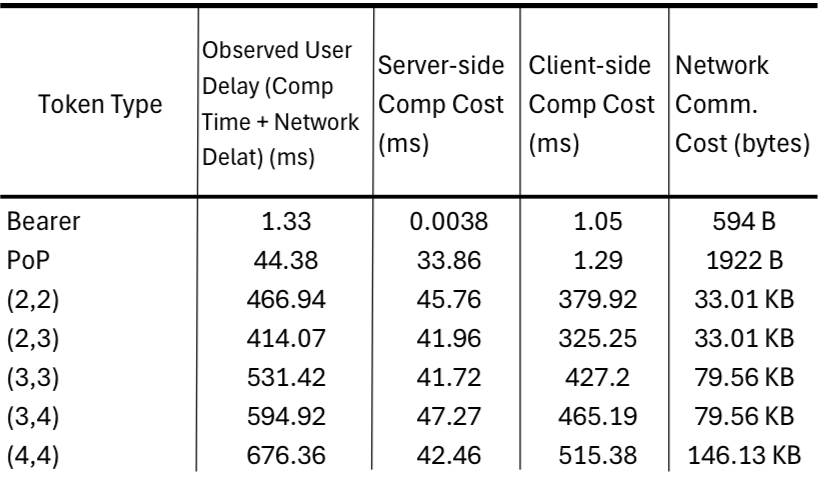
\includegraphics[width=.5\textwidth]{Figures/Results.jpeg}
\caption{Comparison of different token types.}
\label{experiment-table}
\end{centering}
\end{figure}

\noindent{\bf \textit{Experiment Environment and Setup}.}
Our experiments investigate the resource costs of PbDTV so we do not implement user Registration or Token Request phases. Our artifact is a python lirary that implements the Token Showing phase including the SS-NIZK proofs %and a library for PbDTV clients and servers. 
We use our libraries and a simulated LAN network setting and run our experiments on a i7 Intel  16 virtual-core 2.90 GHz CPU and 20 Gb RAM with Ubuntu 20.04.6 LTS. They clients and servers communicate via TCP on the loopback interface. Each node runs on a separate core (\texttt{taskset} command) and we simulate LAN settings by adding 0.1ms delay delays and 10Gbps bandwidth limits (\texttt{tc} command). %The LAN simulations use a rate of  with . %and WAN simulations use 40Mbps rate and 80ms delay like the experiment setup in [4].  

For tokens we use JSON Web Signatures (JWS) \cite{jws-rfc7515} %a subset of JWTs 
used in \cite{openIDConnect,rfc6749OAuth2.0}. The JWS consist of a header, payload, and signature. The payload can be arbitrary bytes and the header is a JSON object that describes the signature algorithm used to sign base64 encodings of the header and payload. Our libraries use NIST’s 2048-bit modular exponential Diffie-Hellman group. We use \cite{pycrypto}'s large integer arithmetic interface for General Multi-Percision library through an interface in and the keccak-based hash function KangarooTwelves \cite{Bertoni2018KangarooTwelveFH}.

We record the time spent by each entity performing local computations as well as the total user delay from start of a request to finish, i.e. receiving the verification result. This includes the time spent in local computation and network delays. We also report the total number of bytes transmitted over all channels for each experiment. 

\noindent \textbf{Bearer Token Implementation.} We use TLS 1.2 between a client and single RP server. The token's payload is a JSON object with username and expiration date values. The protocol is 1 round to send token to the server and receive an accept response. %It is by far the most efficient implementation of tokens, but requires secure handling and has no protections against token stealing.


\noindent \textbf{PoP Token Implementation.} This implementation is based on a 2-round challenge-response protocol \cite{rfc8705} between a client node and a single server. The protocol uses two JWS tokens. One is the ``issued" authentication with username and an RSA 2048-bit public key in its payload and sent to the RP in the first round. The RP sends a random challenge to the client in the second round who uses it as the payload of a new JWS signed with their private key. The new JWS is returned to the RP who verifies it with the pubic-key from the first token.

\noindent \textbf{PbDTV Implementation.}
We build PbDTV systems with different values for $n$ and $t$ shown in Table \ref{experiment-table}. Token verification takes 2-rounds between the client and $t$ servers and a 3-round sub-protocol between the $t$ servers. We record the slowest of the $t$ servers in our results.

\noindent{\bf Results.}
The results are collected in Table \ref{experiment-table} and are the average of 100 runs of the experiments. In our final version we will include detailed error ranges. Our observations follow our expectations in efficiency for the RP. Showing PoP tokens is slower %($\sim32$) 
than showing BT tokens and takes, 44.3 ms and 1.3 ms respectively a %$\sim32$ fold increase, 
and requires roughly double the amount of bytes sent over the network, $\sim1$KB and $\sim0.5$B. PbDTV token showing for experiment $(3, 2)$ is  slower still at almost half a second, 466.94 ms, and requires about 33KB total transmitted bytes. %$\sim54$ times more bytes over the network. Comparing the (3, 2) PbDTV scheme to PoP tokens, our scheme is $\sim8$ times slower and requires the exchange of $\sim16$  times more bytes. 

{\em The PbDTV overhead compared to BT tokens is the cost of protection against token stealing, and compared to PoP tokens is the cost of not requiring secure client storage.} The results suggest that, from a user’s experience point of view, the extra time for verification would be a reasonable trade-off when the user does not have access to secure storage on their device and requires protection against token stealing. This is a common setting when a user wants to log on to a system from a public and trusted terminal (e.g. a University lab or library).

We note that the user device in PoP tokens spends more time performing local computations than the server does, where in our scheme the reverse is true. In fact the user’s computational time for PbDTV tokens remains fairly static for different values of $n$ and $t$ and user’s local computation in the (4, 4) experiment is only \%25 longer than that PoP tokens. {\em This suggests that our PbDTV scheme can be used by a wider range of user devices than the PoP tokens.} While both schemes require devices with comparable computing power PbDTV does not require a secure storage module like the PoP does.  

\noindent{\textbf{Comparison to distributed token generation}}. Distributed token generation in \cite{PASTA-Agrawal} %[4] 
and \cite{PESTO-baum} %[7] is 
are significantly more efficient than distributed verification. For example the issuing time for a $(3,2)$ token generation in PASTA is 14.5 ms with similar simulation settings. This is because in PbDTV no password related data is stored on verification servers and the users are only required to register with the authentication server(s) (centralized or distributed).  
%This is an important operational requirement and allows the users to register only once, and enjoy protection against token stealing by any group of verification servers that is willing to provide the service to the authentication sever(s). Verification in this setting is a distributed process and requires extra computation and communication.



\section{Conclusion \& Future Work}
\label{sec:Conclusion}
We presented two extensions to 
password-based token generation and secure token showing with protection against token stealing.
%protocols.
The two systems can be used individually with other public-key based token systems. For example PbDTV allows $pwd_v$ be used instead of the user's public key in today's SSO systems, and PASCA can be used with embedded public key in the token for protection against token stealing.
%can be used instead of PoP protocol
An important aspect of our work in securing SSO systems is using only passwords and removing the need for secure storage on the device for %to safely 
obtaining and presenting tokens. %We also introduced the notion of ring-token-anonymity that enables a user to have some level of anonymity against the $IdP$. We argued that the additional computation and communication cost of the system suggests offering it as a paid service, which has the additional benefit of being abused for DOS attacks.
%at the costfor token requests. 
Interesting direction for future work are more efficient constructions and constructions with post-quantum security.
%future work would be to find more efficient ways to achieve our goals and to extend privacy to the token showing protocol.

%%
%% Print the bibliography
%%
%\printbibliography
\bibliographystyle{splncs04}
\bibliography{mybibliography1}


%\section{Conclusion}
%The conclusion goes here.




% conference papers do not normally have an appendix


% use section* for acknowledgment
%\section*{Acknowledgment}
%

%The authors would like to thank...





% trigger a \newpage just before the given reference
% number - used to balance the columns on the last page
% adjust value as needed - may need to be readjusted if
% the document is modified later
%\IEEEtriggeratref{8}
% The "triggered" command can be changed if desired:
%\IEEEtriggercmd{\enlargethispage{-5in}}

% references section

% can use a bibliography generated by BibTeX as a .bbl file
% BibTeX documentation can be easily obtained at:
% http://mirror.ctan.org/biblio/bibtex/contrib/doc/
% The IEEEtran BibTeX style support page is at:
% http://www.michaelshell.org/tex/ieeetran/bibtex/
%\bibliographystyle{IEEEtran}
% argument is your BibTeX string definitions and bibliography database(s)
%\bibliography{IEEEabrv,../bib/paper}
%
% <OR> manually copy in the resultant .bbl file
% set second argument of \begin to the number of references
% (used to reserve space for the reference number labels box)
\begin{thebibliography}{1}

\bibitem{IEEEhowto:kopka}
H.~Kopka and P.~W. Daly, \emph{A Guide to \LaTeX}, 3rd~ed.\hskip 1em plus
  0.5em minus 0.4em\relax Harlow, England: Addison-Wesley, 1999.

\end{thebibliography}




% that's all folks
\end{document}


